\section{Apéndice}

\subsection{Registro y Login}

\begin{figure}[H]
    \centering
    
\includegraphics[width=0.75\linewidth]{Documento Final/Imagenes/LogIn.jpg}
    \caption{Página de inicio de sesión de UnaCloud, donde los usuarios ingresan sus credenciales para acceder a la plataforma.}
    \label{fig:LogIn}
\end{figure}

\begin{figure}[H]
    \centering
    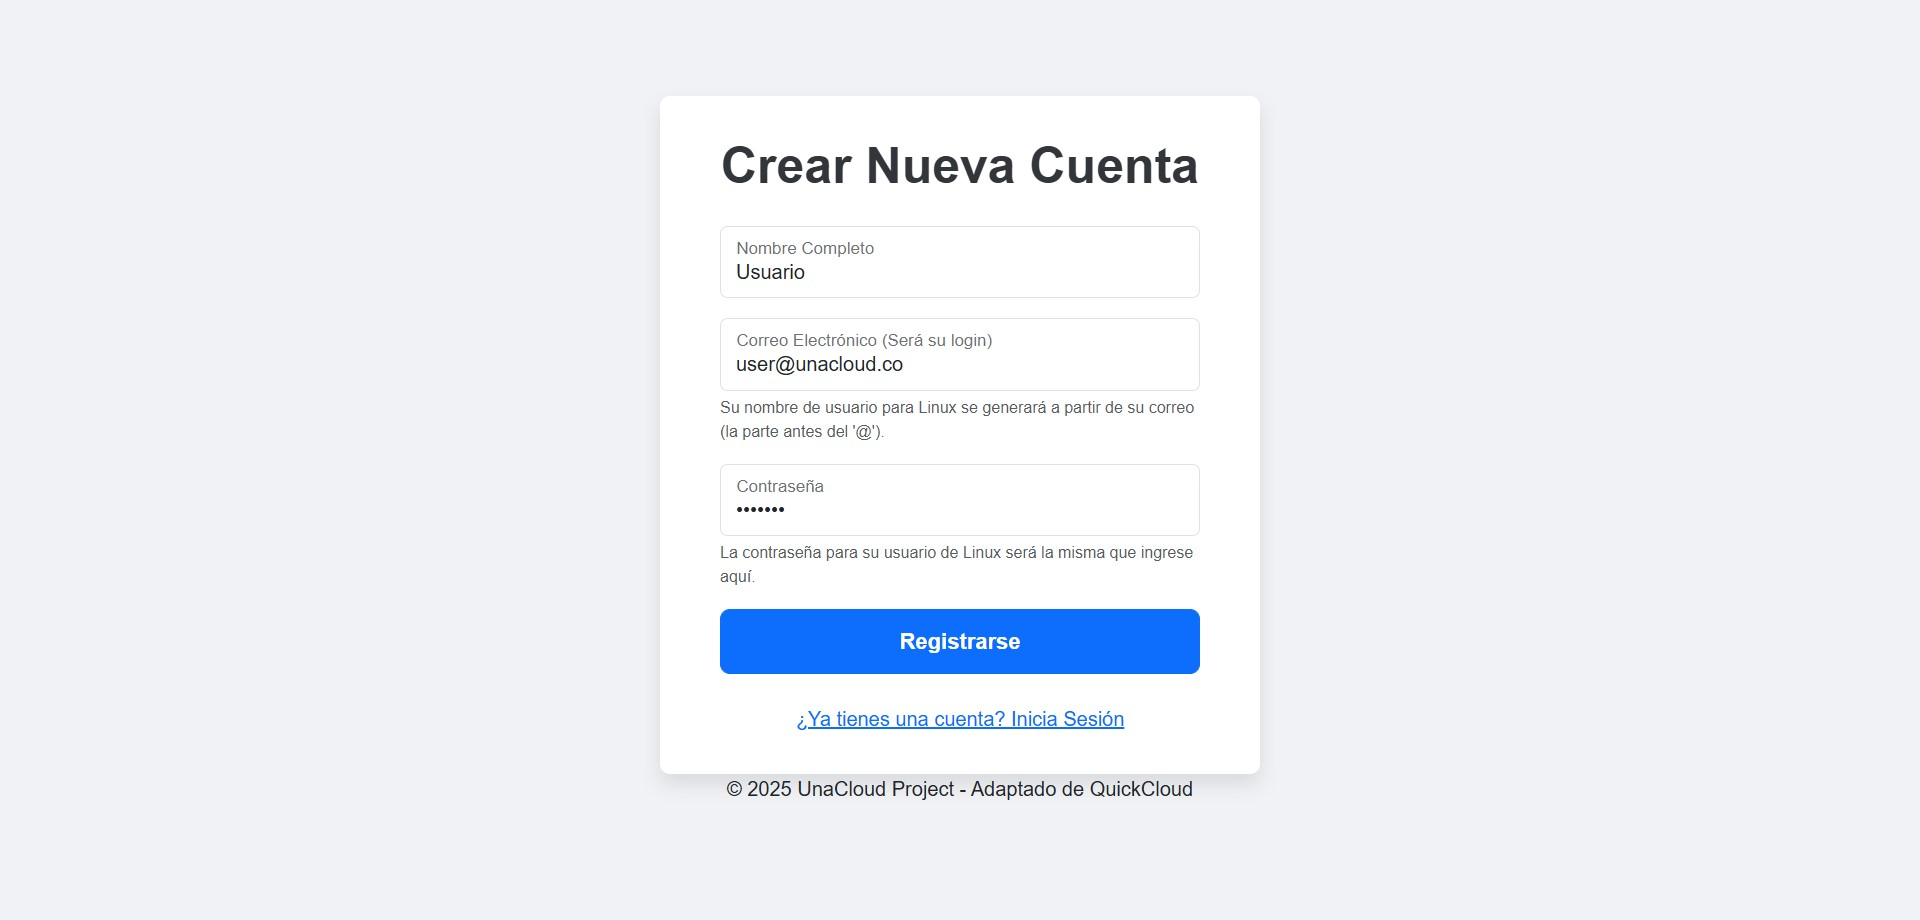
\includegraphics[width=0.75\linewidth]{Documento Final/Imagenes/Register.jpg}
    \caption{Interfaz de registro de nuevos usuarios. Se solicita el nombre completo, correo electrónico y contraseña. El sistema informa que el nombre de usuario en Linux se generará a partir del correo y que la contraseña será la misma para ambos sistemas.}
    \label{fig:SignUp}
\end{figure}

\begin{figure}[H]
    \centering
    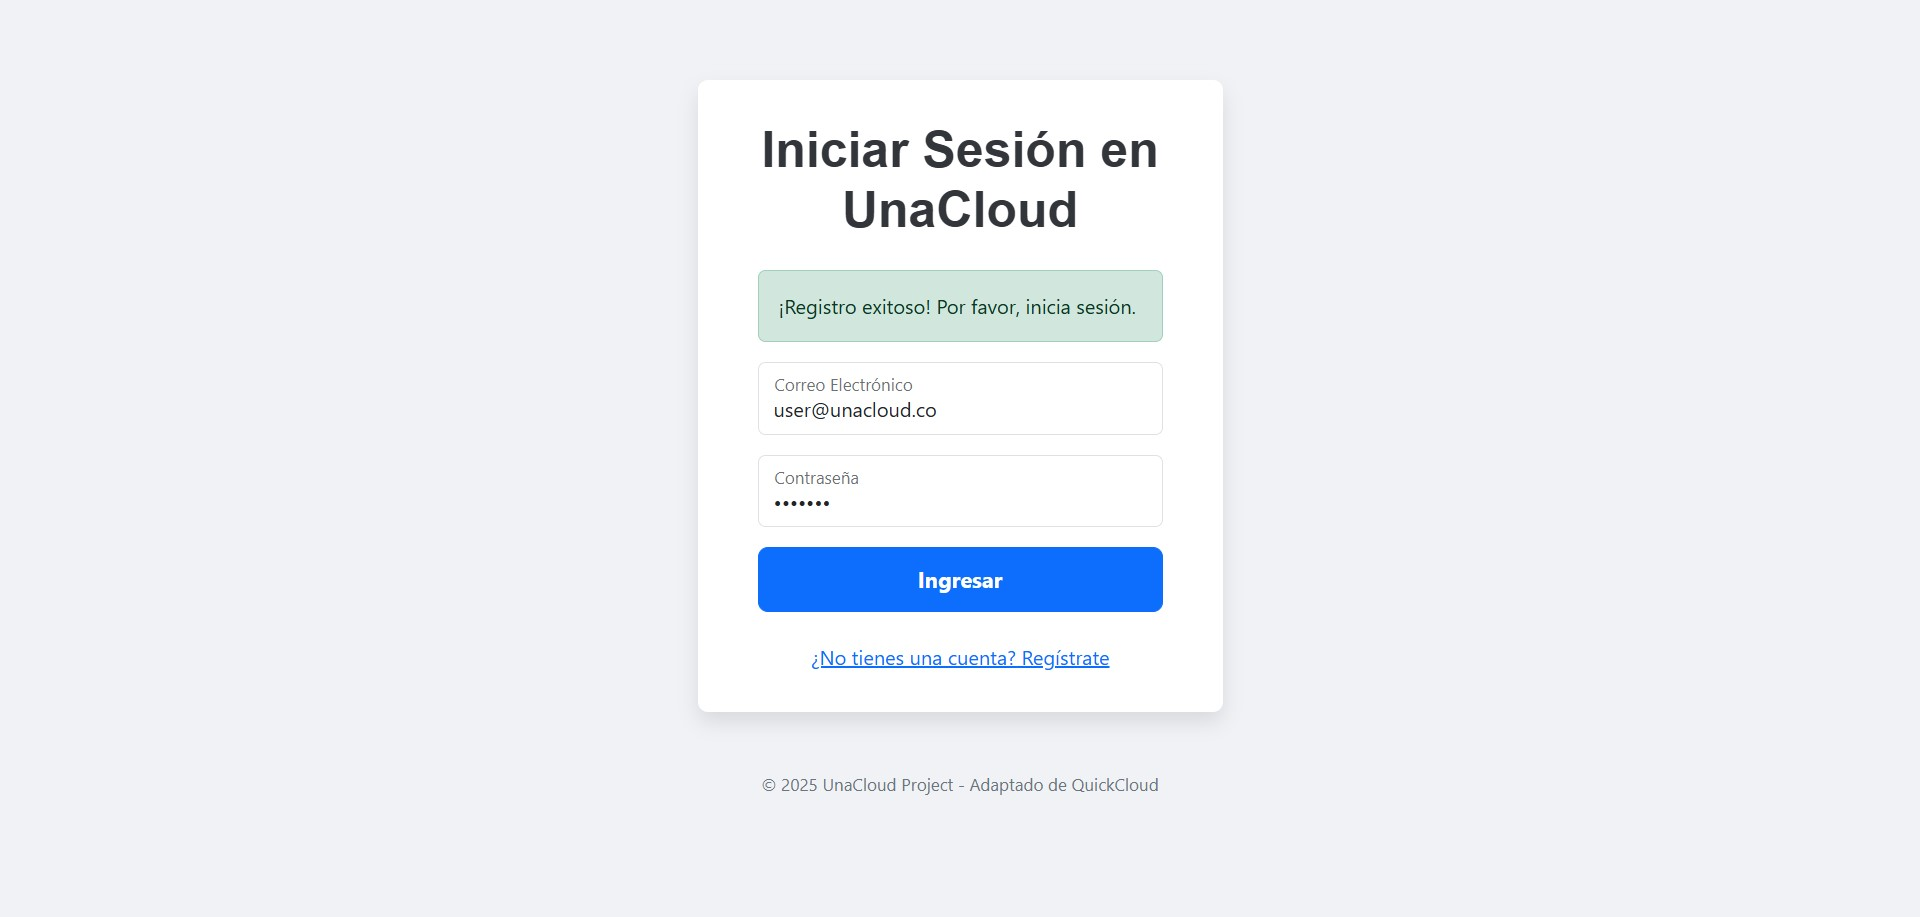
\includegraphics[width=0.75\linewidth]{Documento Final/Imagenes/LoginConRegistro.jpg}
    \caption{Vista de la página de inicio de sesión que muestra un mensaje de confirmación al usuario después de haberse registrado exitosamente, invitándolo a ingresar por primera vez.}
    \label{fig:LogIn2}
\end{figure}

\begin{figure}[H]
    \centering
    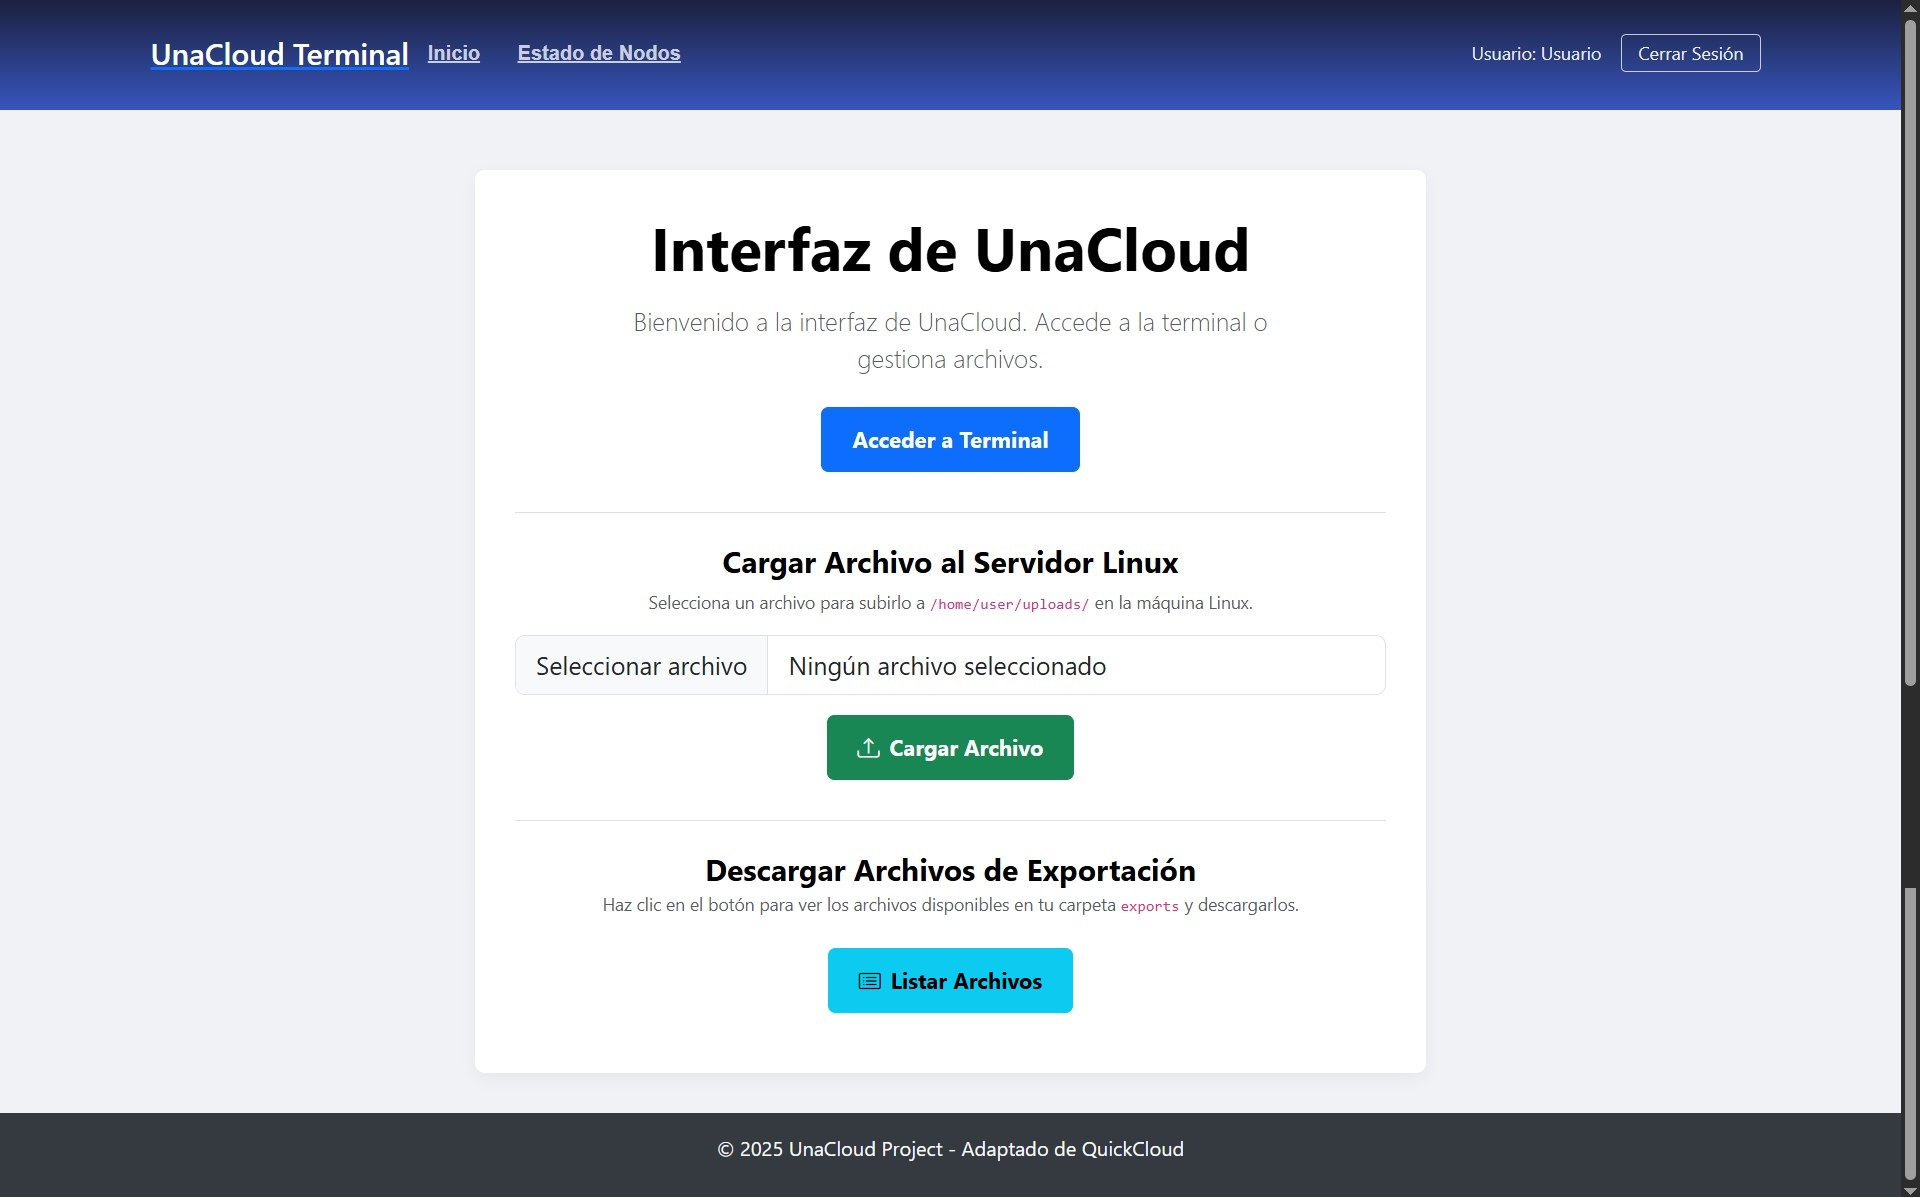
\includegraphics[width=0.75\linewidth]{Documento Final/Imagenes/HomePageUser.jpg}
    \caption{Vista principal de la aplicación después de que un usuario ha iniciado sesión. Muestra las funcionalidades disponibles, incluyendo el acceso a la terminal, la carga de archivos al servidor Linux y la descarga de archivos de exportación.}
    \label{fig:LogedIn}
\end{figure}

\subsection{Funcionalidades de la página de inicio}

\begin{figure}[H]
    \centering
    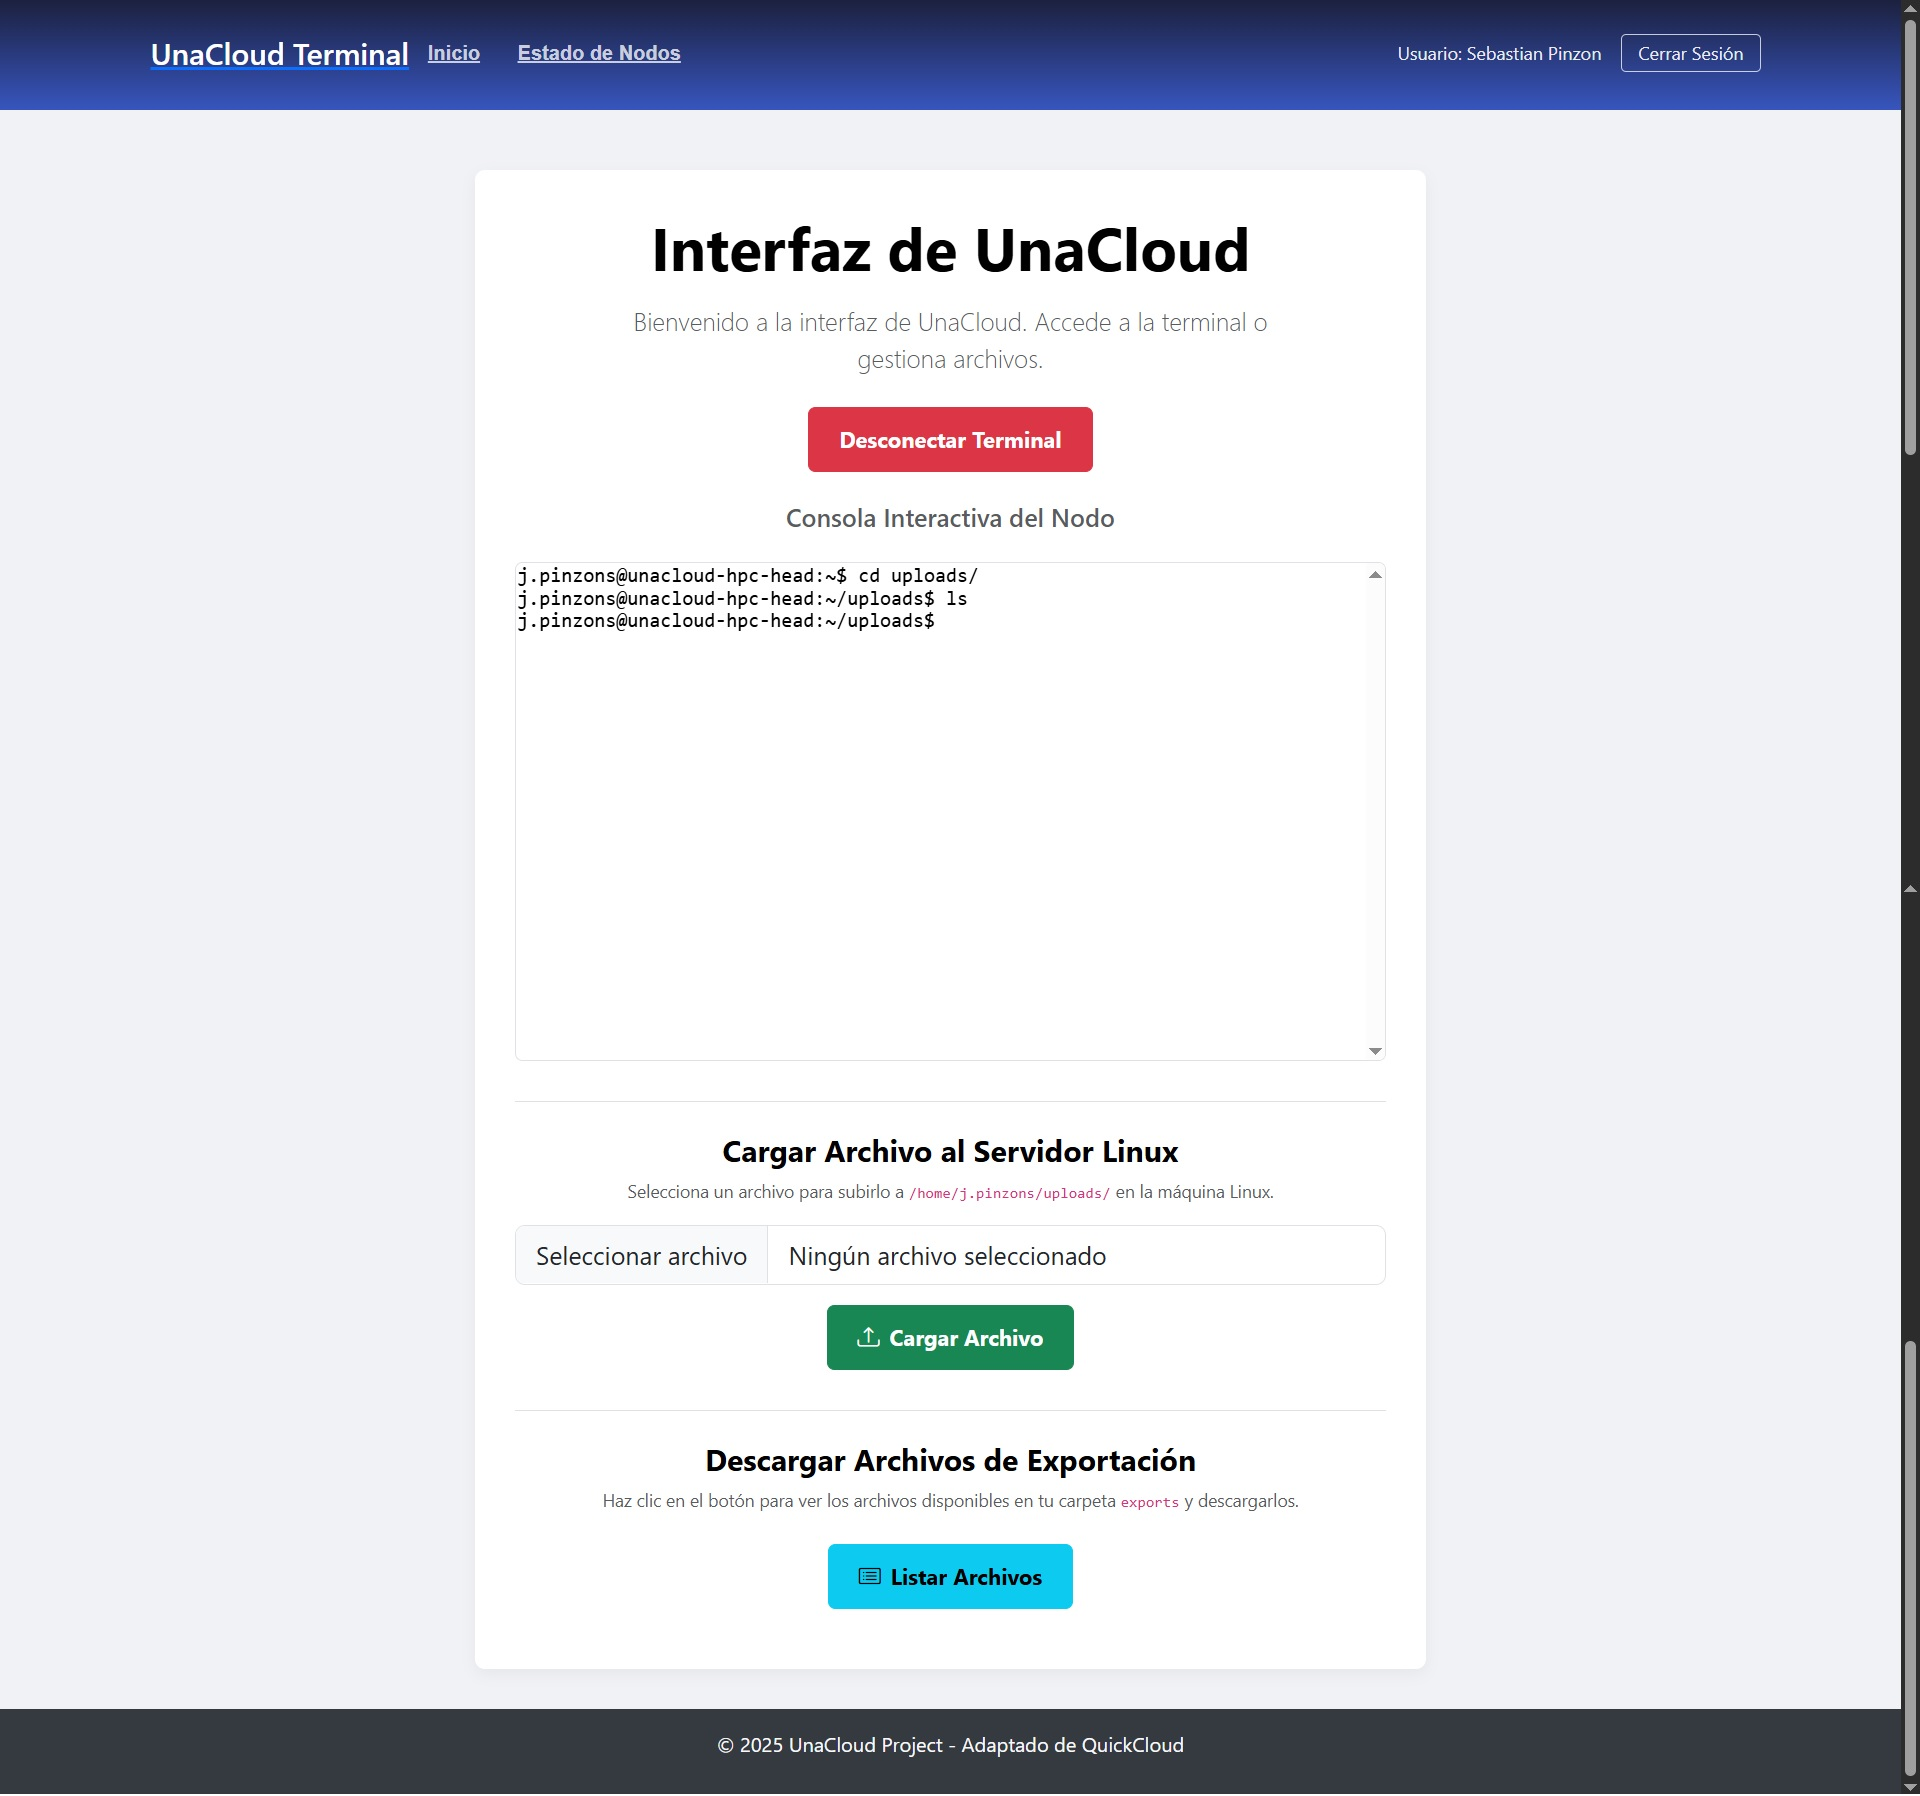
\includegraphics[width=0.75\linewidth]{Documento Final/Imagenes/EmptyUploads.jpg}
    \caption{Un investigador accede a su directorio de trabajo (/uploads) a través de la terminal web. Inicialmente, el directorio se encuentra vacío, listo para recibir los archivos del trabajo de investigación.}
    \label{fig:EmptyUpload}
\end{figure}

\begin{figure}[H]
    \centering
    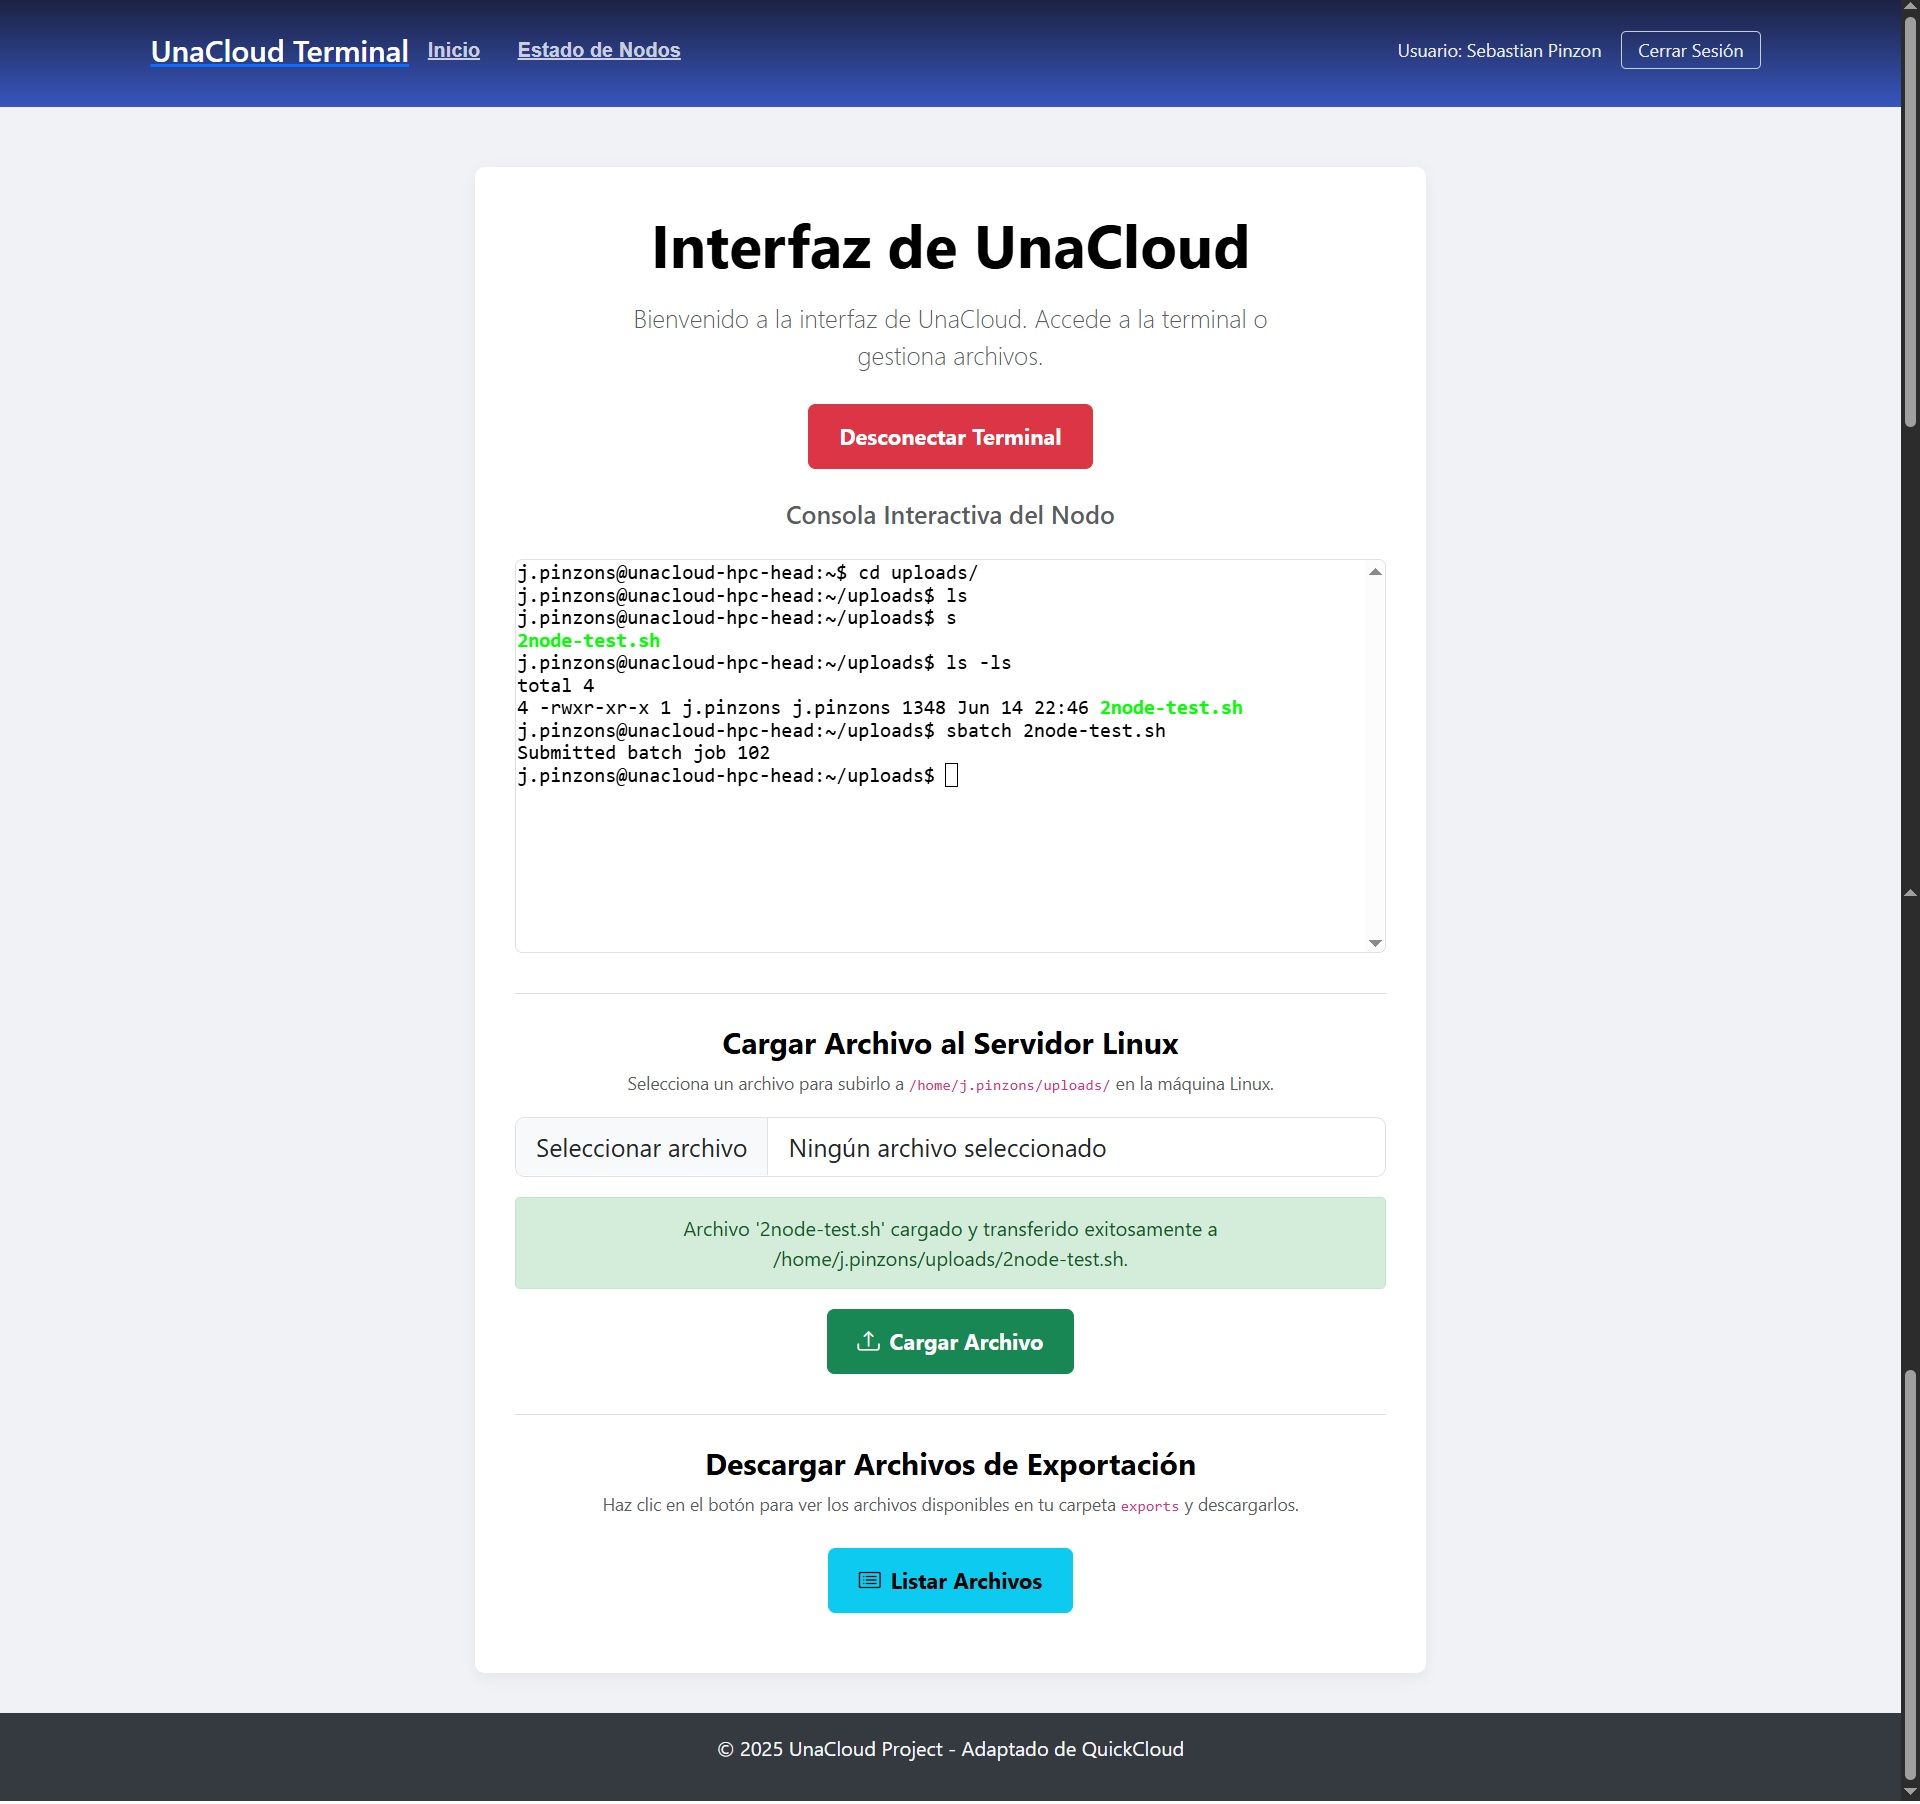
\includegraphics[width=0.75\linewidth]{Documento Final/Imagenes/RunningTask.jpg}
    \caption{Después de cargar su script (2node-test.sh) a través de la interfaz, el investigador lo envía a la cola de procesamiento de Slurm usando el comando sbatch. El sistema confirma la recepción del trabajo con el ID de lote 102.}
    \label{fig:RunningTask}
\end{figure}

\begin{figure}[H]
    \centering
    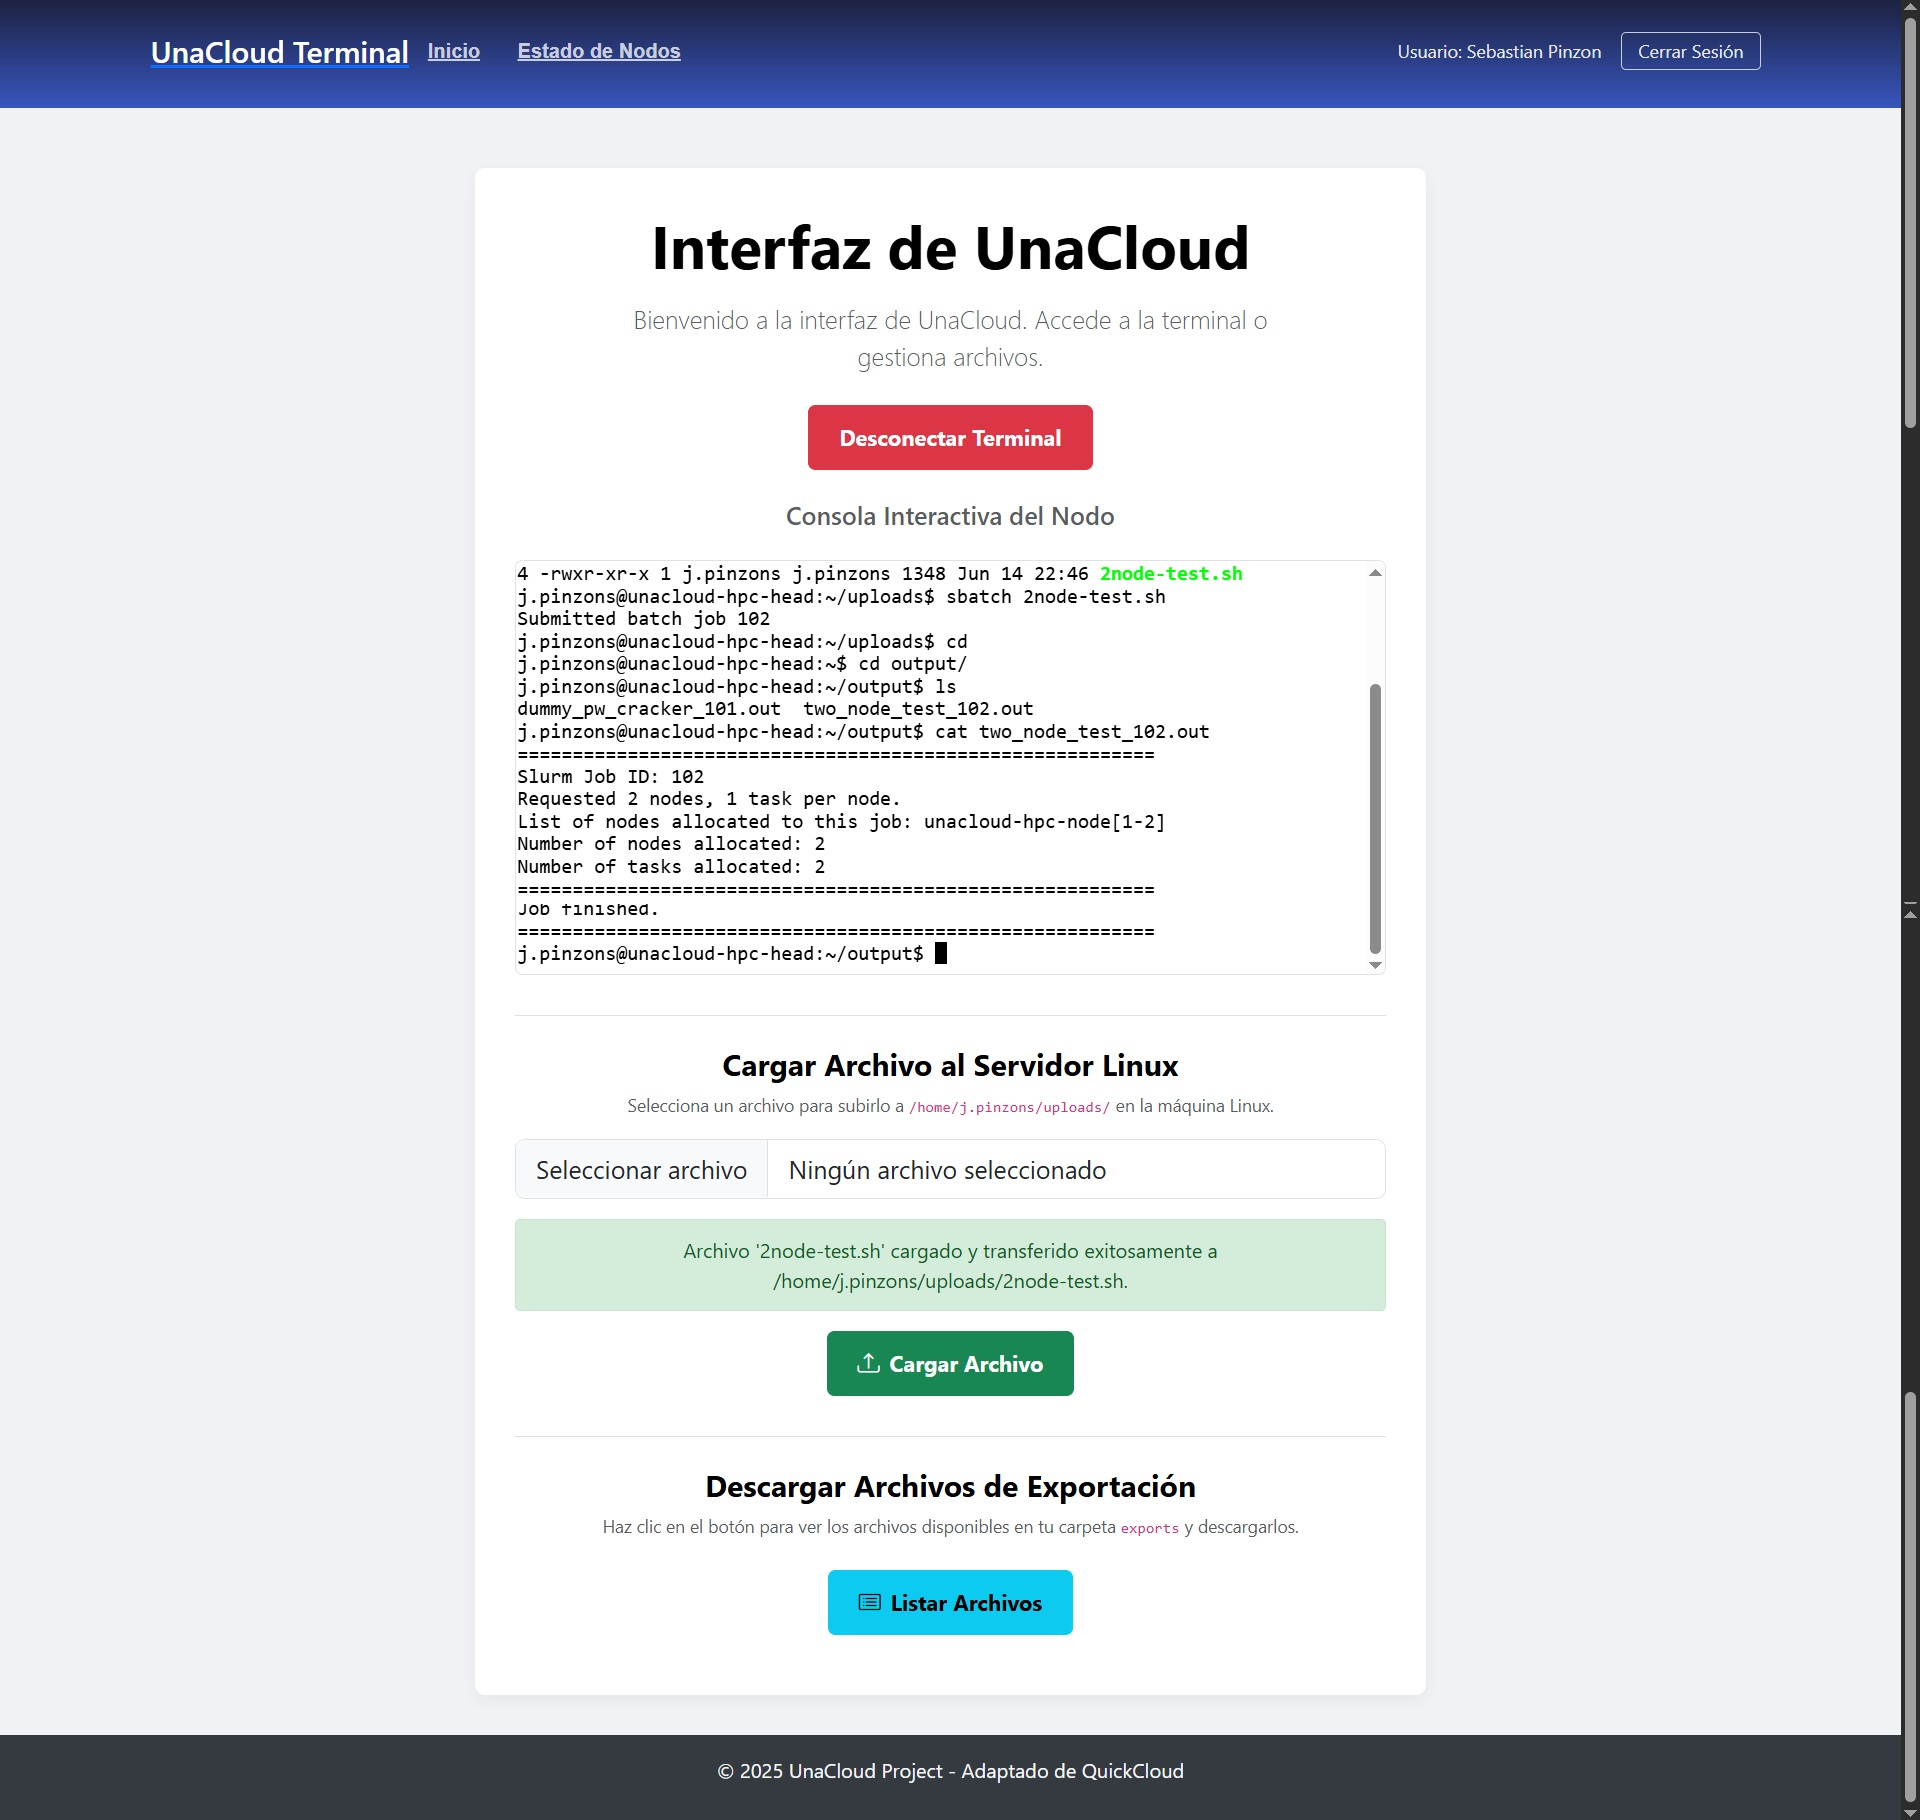
\includegraphics[width=0.75\linewidth]{Documento Final/Imagenes/TaskComplete.jpg}
    \caption{El investigador verifica la finalización del trabajo con ID 102. La terminal muestra que se ejecutó en dos nodos (unacloud-hpc-node[1-2]) y que ha finalizado. Además, se visualiza el contenido del archivo de salida.}
    \label{fig:TaskComplete}
\end{figure}

\begin{figure}[H]
    \centering
    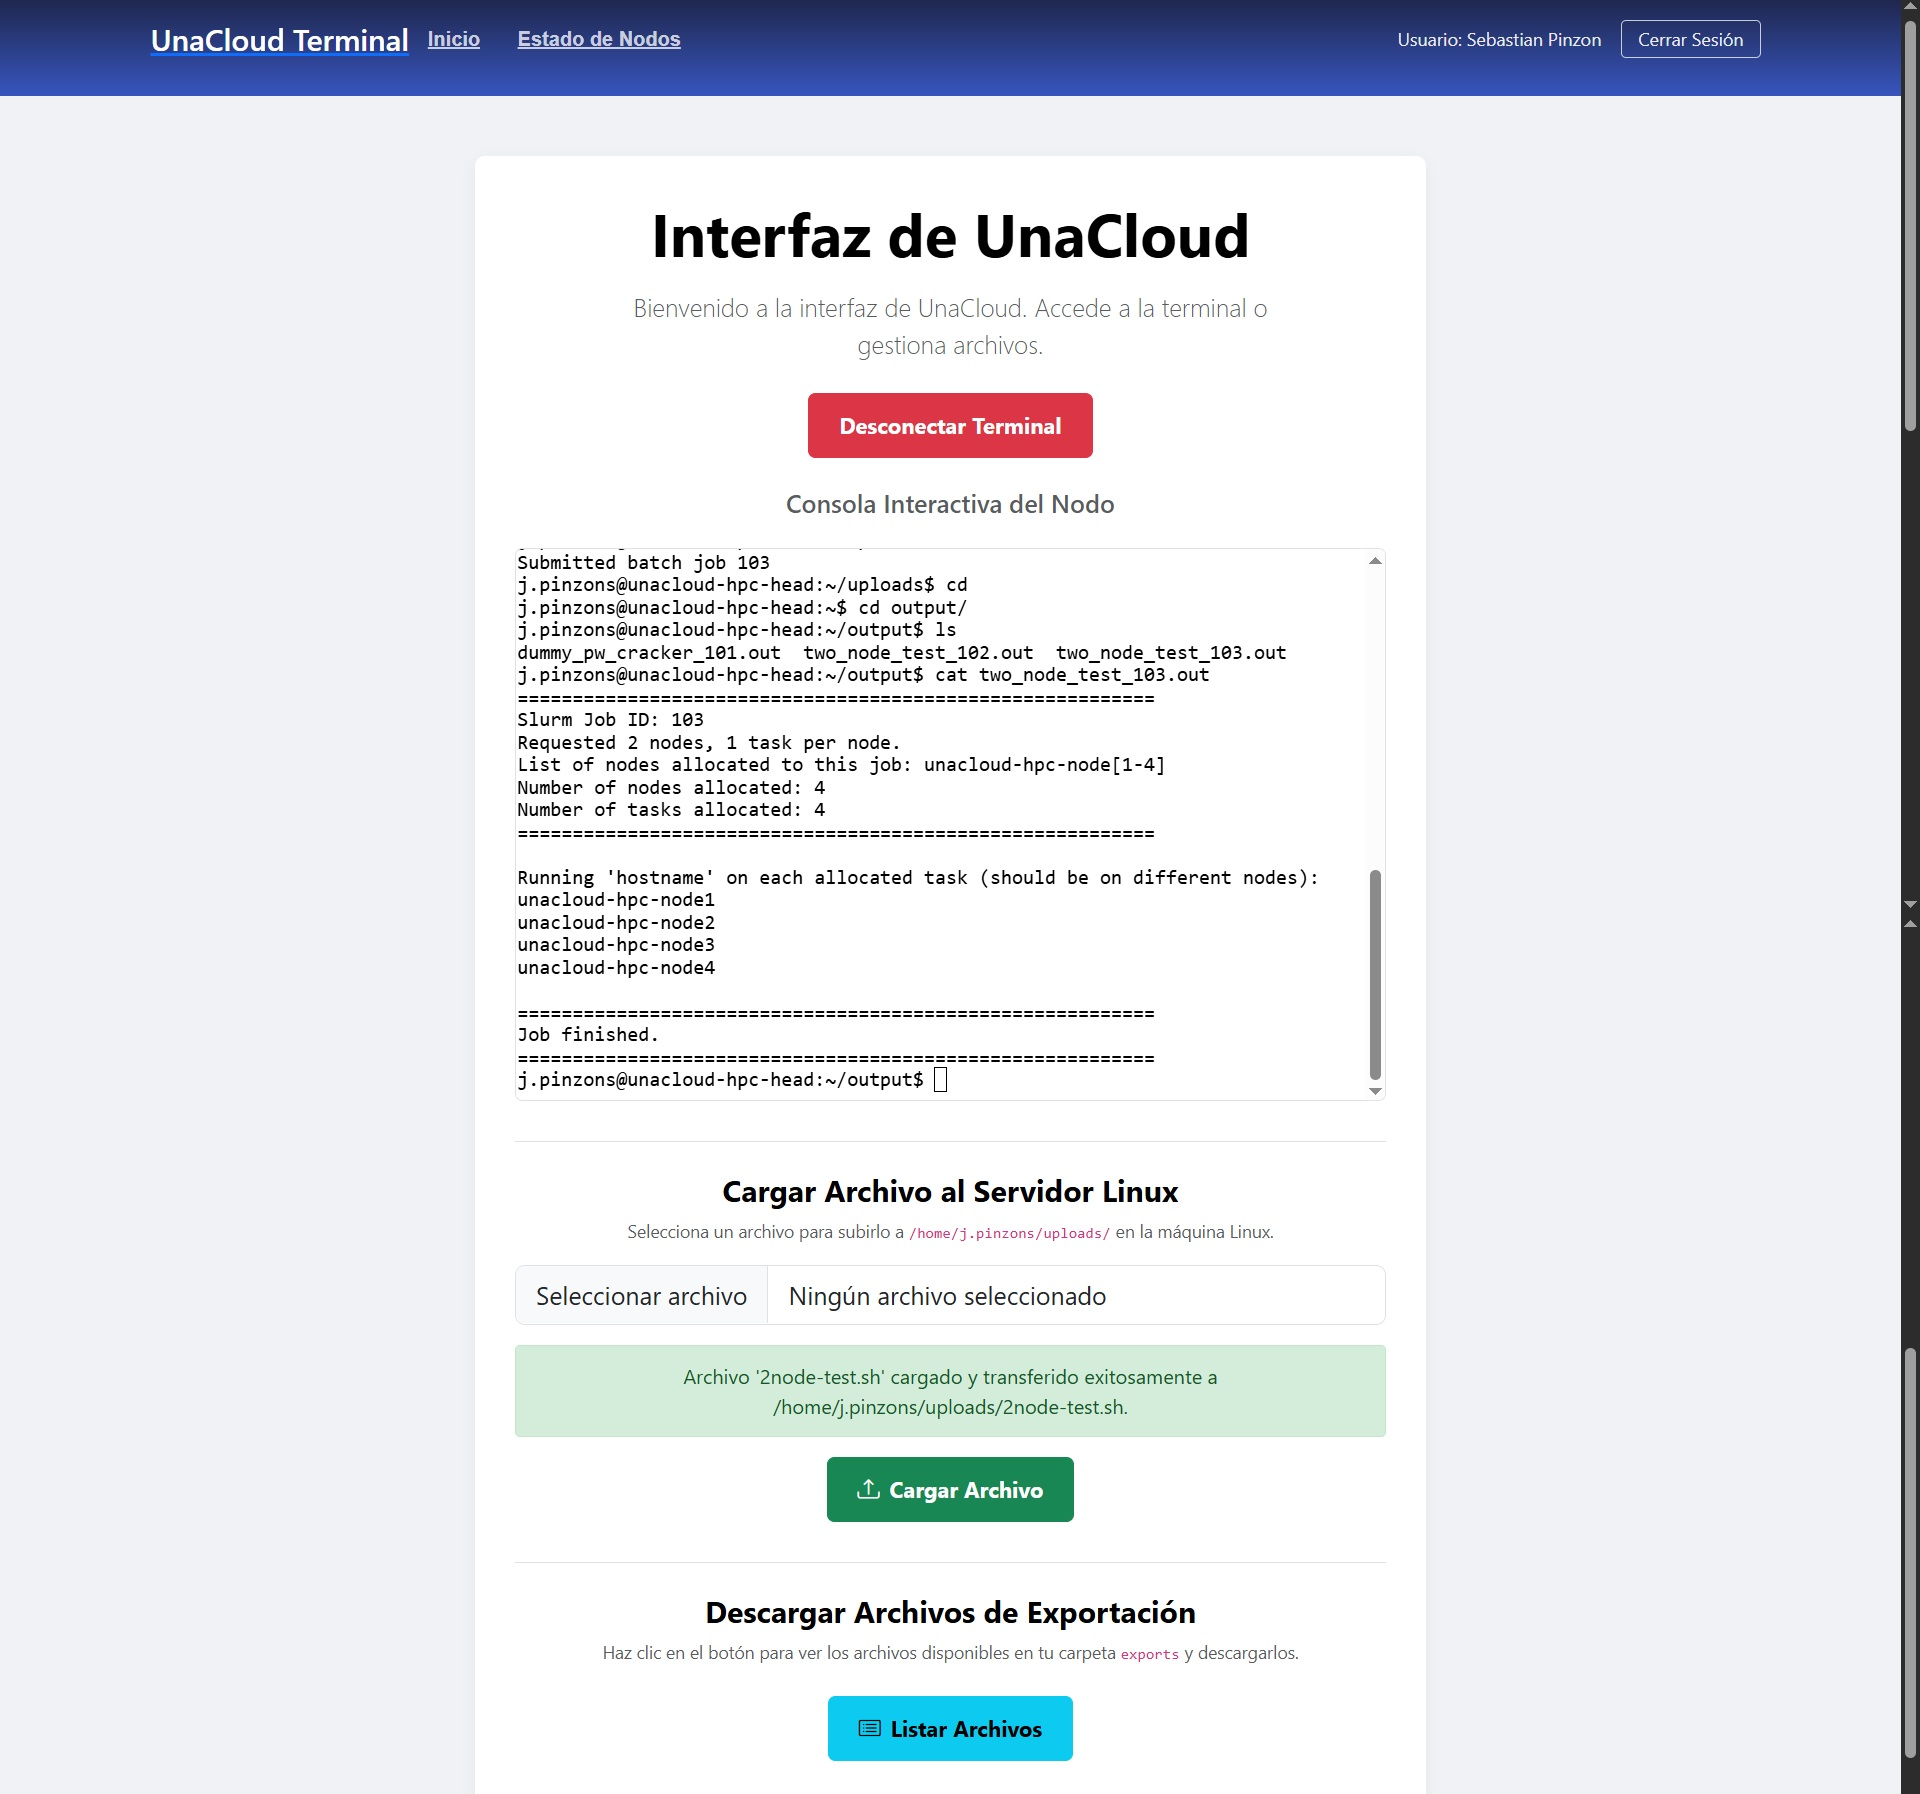
\includegraphics[width=0.75\linewidth]{Documento Final/Imagenes/TaskComplete2.jpg}
    \caption{Muestra la finalización de un trabajo más complejo (ID 103) que se ejecutó en cuatro nodos. La salida del programa confirma la ejecución en paralelo al imprimir el nombre de host de cada nodo (unacloud-hpc-node1 a unacloud-hpc-node4).}
    \label{fig:TaskComplete2}
\end{figure}

\begin{figure}[H]
    \centering
    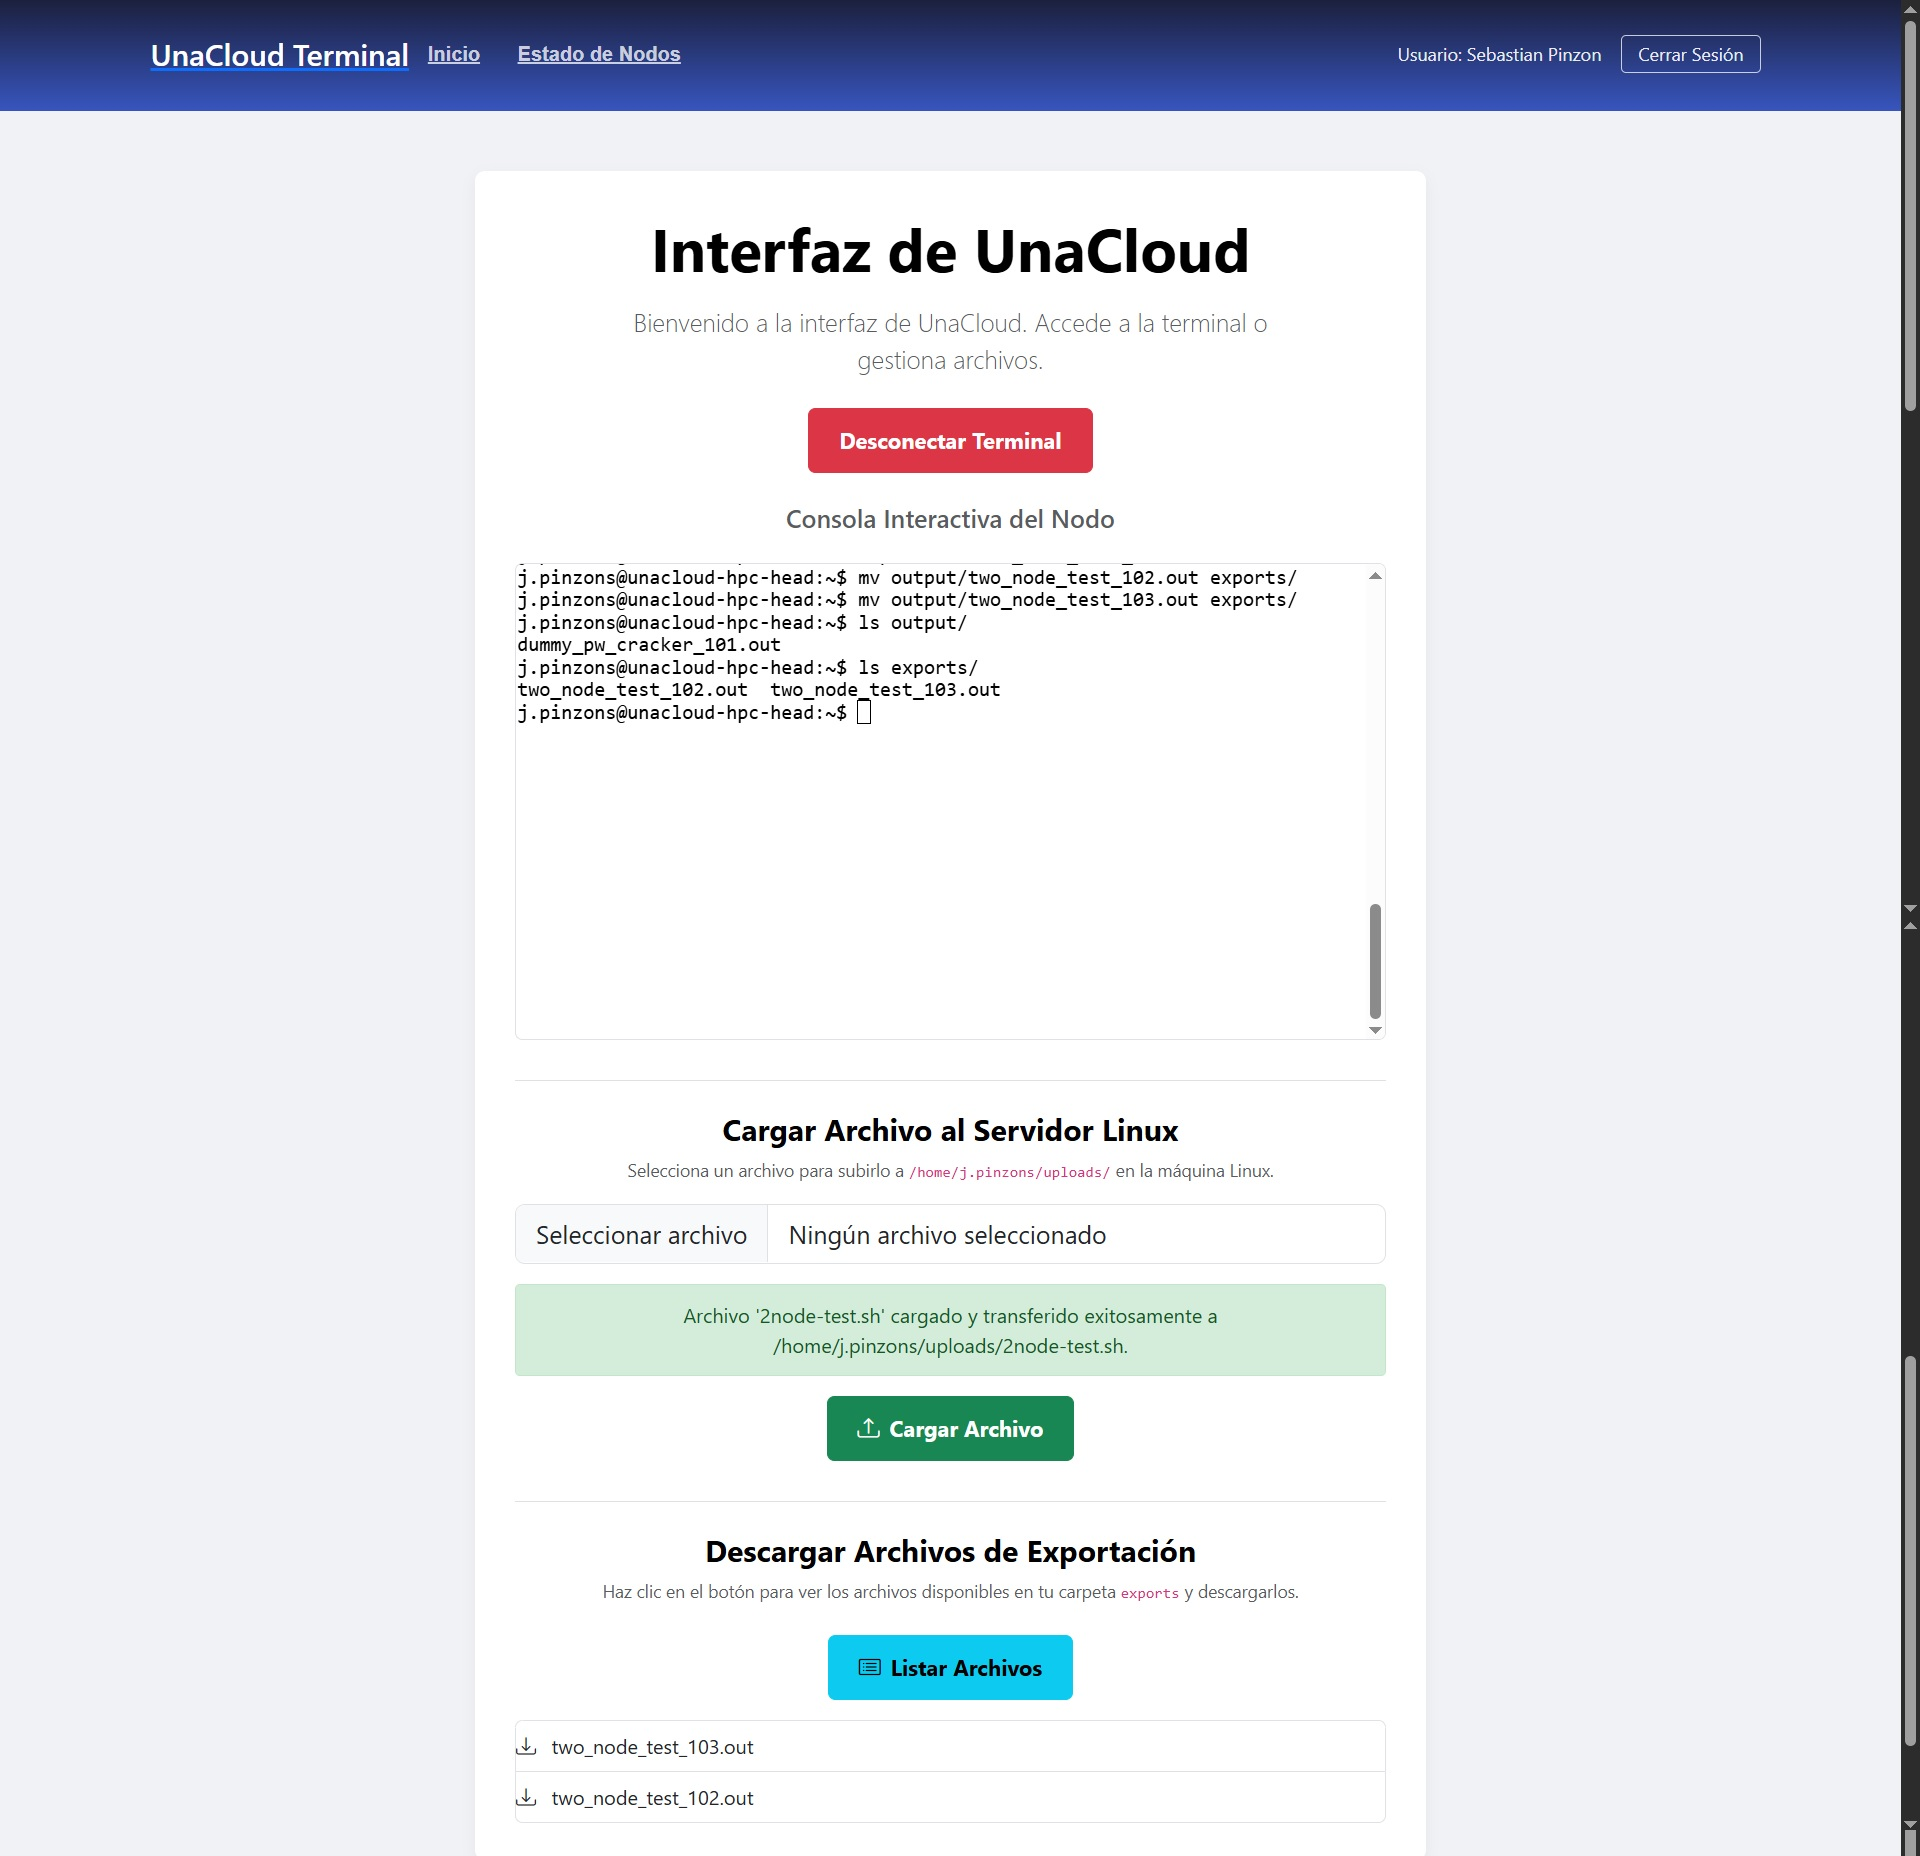
\includegraphics[width=0.75\linewidth]{Documento Final/Imagenes/ExportResults.jpg}
    \caption{El investigador mueve los archivos de salida de sus trabajos a la carpeta exports en la terminal. Al hacer clic en "Listar Archivos", la interfaz web se actualiza y muestra correctamente los archivos, preparándolos para la descarga.}
    \label{fig:ExportResults}
\end{figure}

\begin{figure}[H]
    \centering
    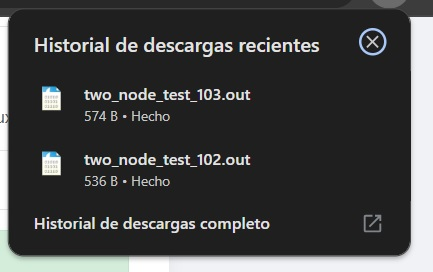
\includegraphics[width=0.75\linewidth]{Documento Final/Imagenes/ExportSuccesfully.jpg}
    \caption{El historial de descargas del navegador confirma que el investigador ha descargado con éxito los archivos de resultados desde la plataforma UnaCloud a su máquina local, completando el ciclo del trabajo de investigación.}
    \label{fig:ExportSuccesfully}
\end{figure}

\subsection{Funcionalidades de la página de estado de nodos}

\begin{figure}[H]
    \centering
    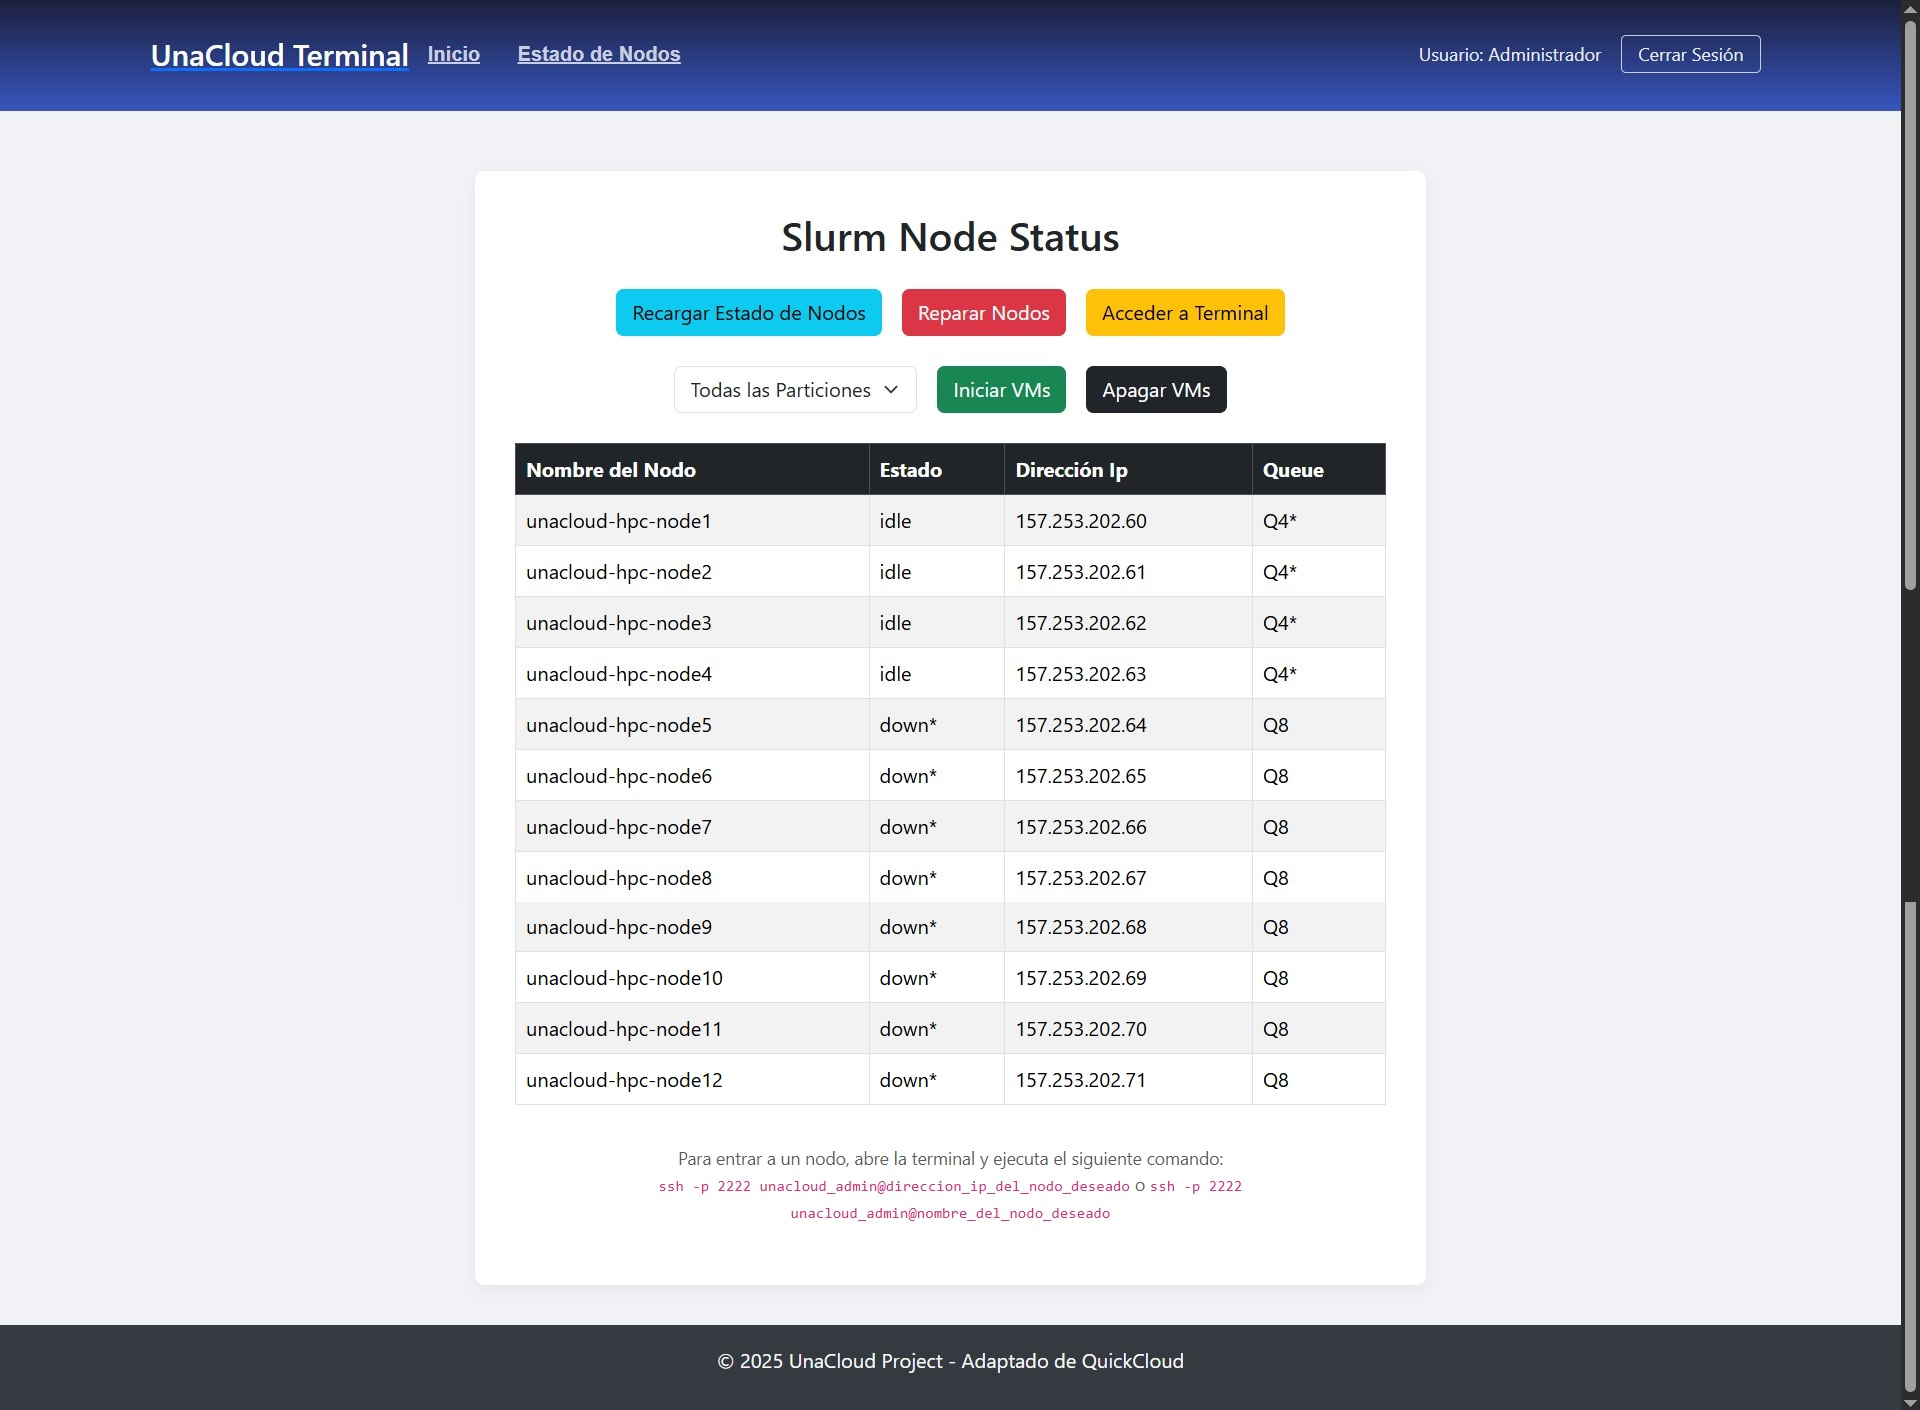
\includegraphics[width=0.75\linewidth]{Documento Final/Imagenes/EstadoNodo_Admin.jpg}
    \caption{Panel de control del administrador que muestra el estado actual de todos los nodos del clúster Slurm. Se observan nodos activos (idle) y otros apagados (down*), junto con opciones para gestionar las particiones, iniciar/apagar VMs y acceder a la terminal.}
    \label{fig:NodeState}
\end{figure}

\begin{figure}[H]
    \centering
    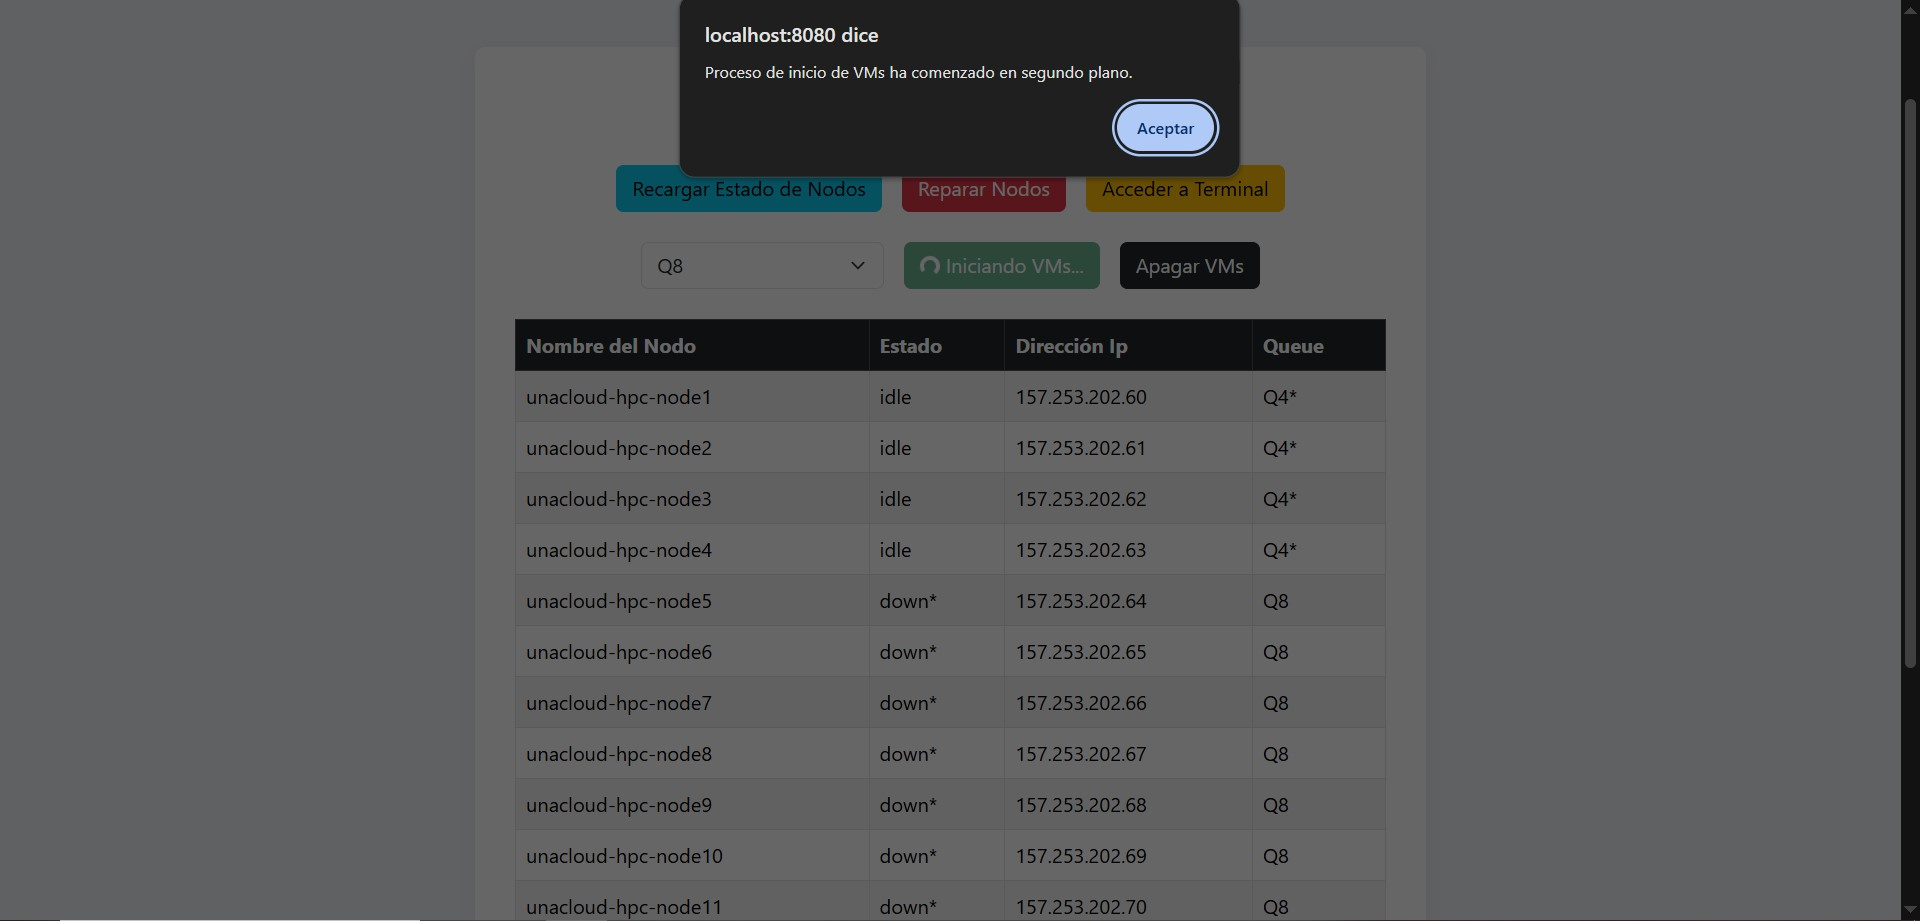
\includegraphics[width=0.75\linewidth]{Documento Final/Imagenes/Vms Q8 iniciadas.jpg}
    \caption{Proceso de inicio de las máquinas virtuales pertenecientes a la partición "Q8". La interfaz muestra una notificación de que el proceso ha comenzado en segundo plano y el botón correspondiente indica "Iniciando VMs...".}
    \label{fig:VMInit}
\end{figure}

\begin{figure}[H]
    \centering
    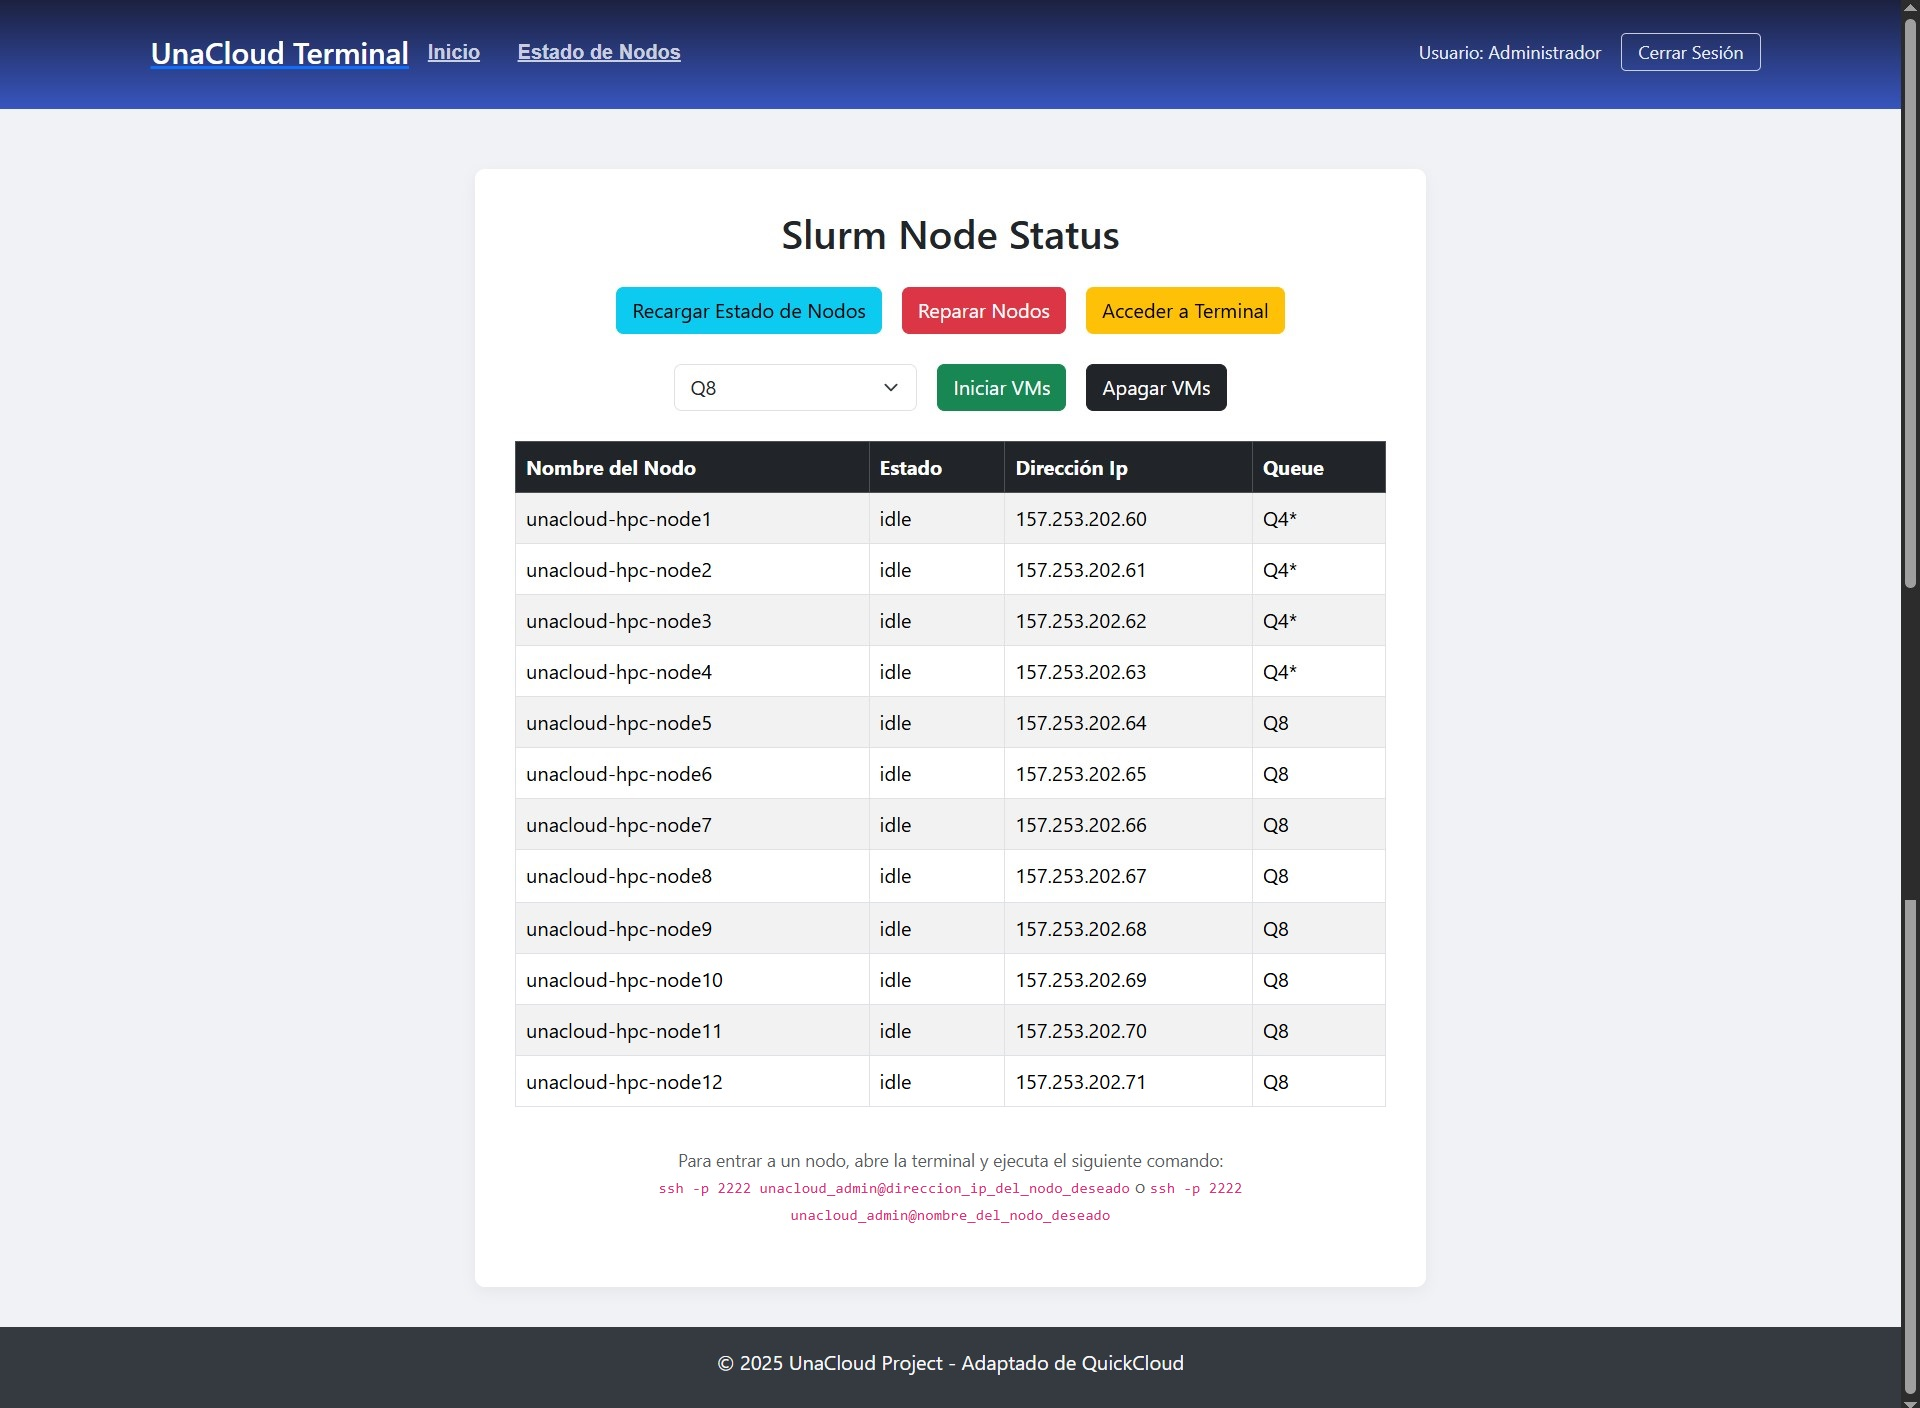
\includegraphics[width=0.75\linewidth]{Documento Final/Imagenes/NodosReparados_admin.jpg}
    \caption{El administrador ha activado la función "Reparar Nodos" desde el panel de control. E inmediatamente se selecciono presiono el botón "Recargar Estado de Nodos", de forma que se puede observar que las maquinas pertenecientes a la partición Q8 fueron prendidas efectivamente y ya se encuentran listas para la realización de una tarea.}
    \label{fig:UCRepair}
\end{figure}

\begin{figure}[H]
    \centering
    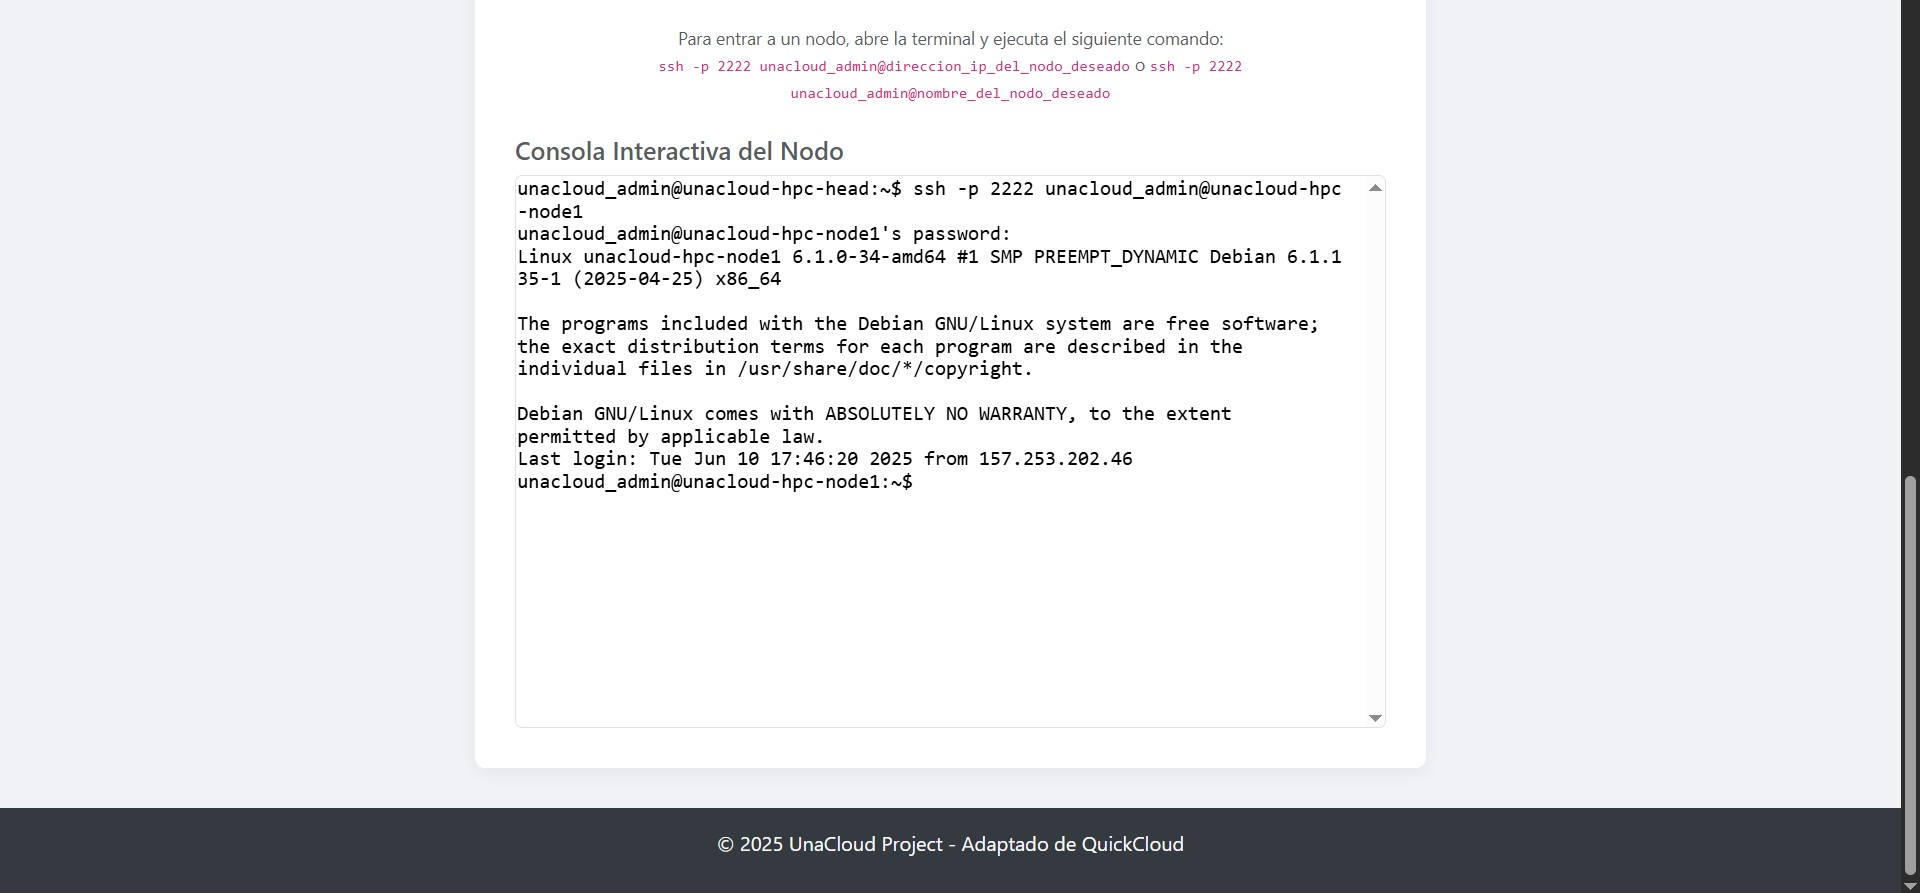
\includegraphics[width=0.75\linewidth]{Documento Final/Imagenes/IngresoANodoPorSSH.jpg}
    \caption{Un administrador utilizando la terminal web para acceder directamente a un nodo de cómputo (unacloud-hpc-node1) a través de SSH. Esto demuestra la capacidad de realizar tareas de mantenimiento avanzadas directamente en los nodos.}
    \label{fig:UCHop}
\end{figure}

\begin{figure}[H]
    \centering
    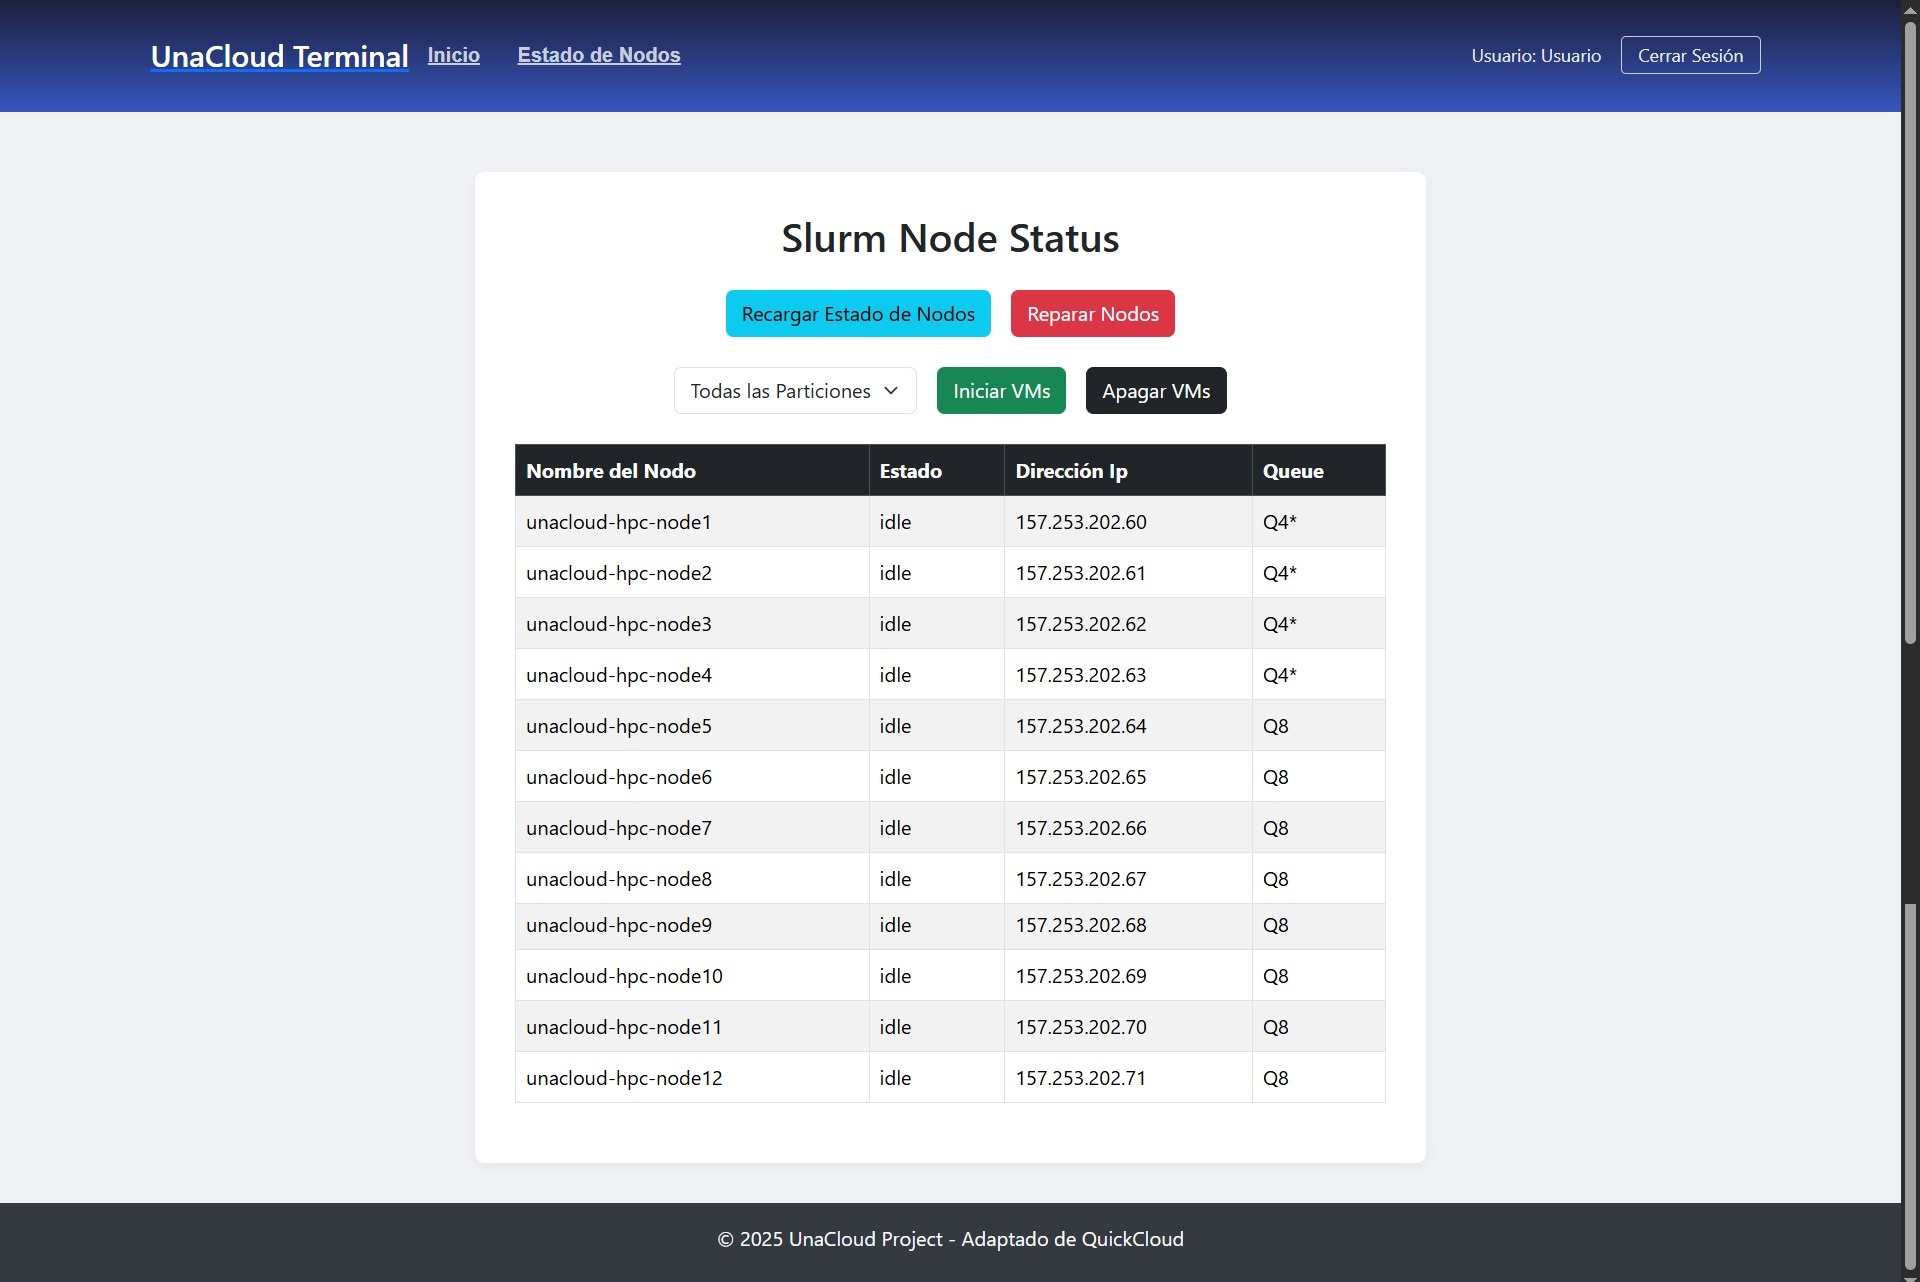
\includegraphics[width=0.75\linewidth]{Documento Final/Imagenes/NodosUser.jpg}
    \caption{Vista del estado del clúster Slurm para un usuario con rol de investigador. El usuario puede ver el estado de los nodos, recargarlos, iniciar maquinas virtuales y apagar las mismas. Sin embargo, no tiene la opción de abrir terminal, ni tampoco posee la información de como conectarse vía SSH a los nodos para repararlos internamente.}
    \label{fig:UCUser}
\end{figure}

\begin{figure}[H]
    \centering
    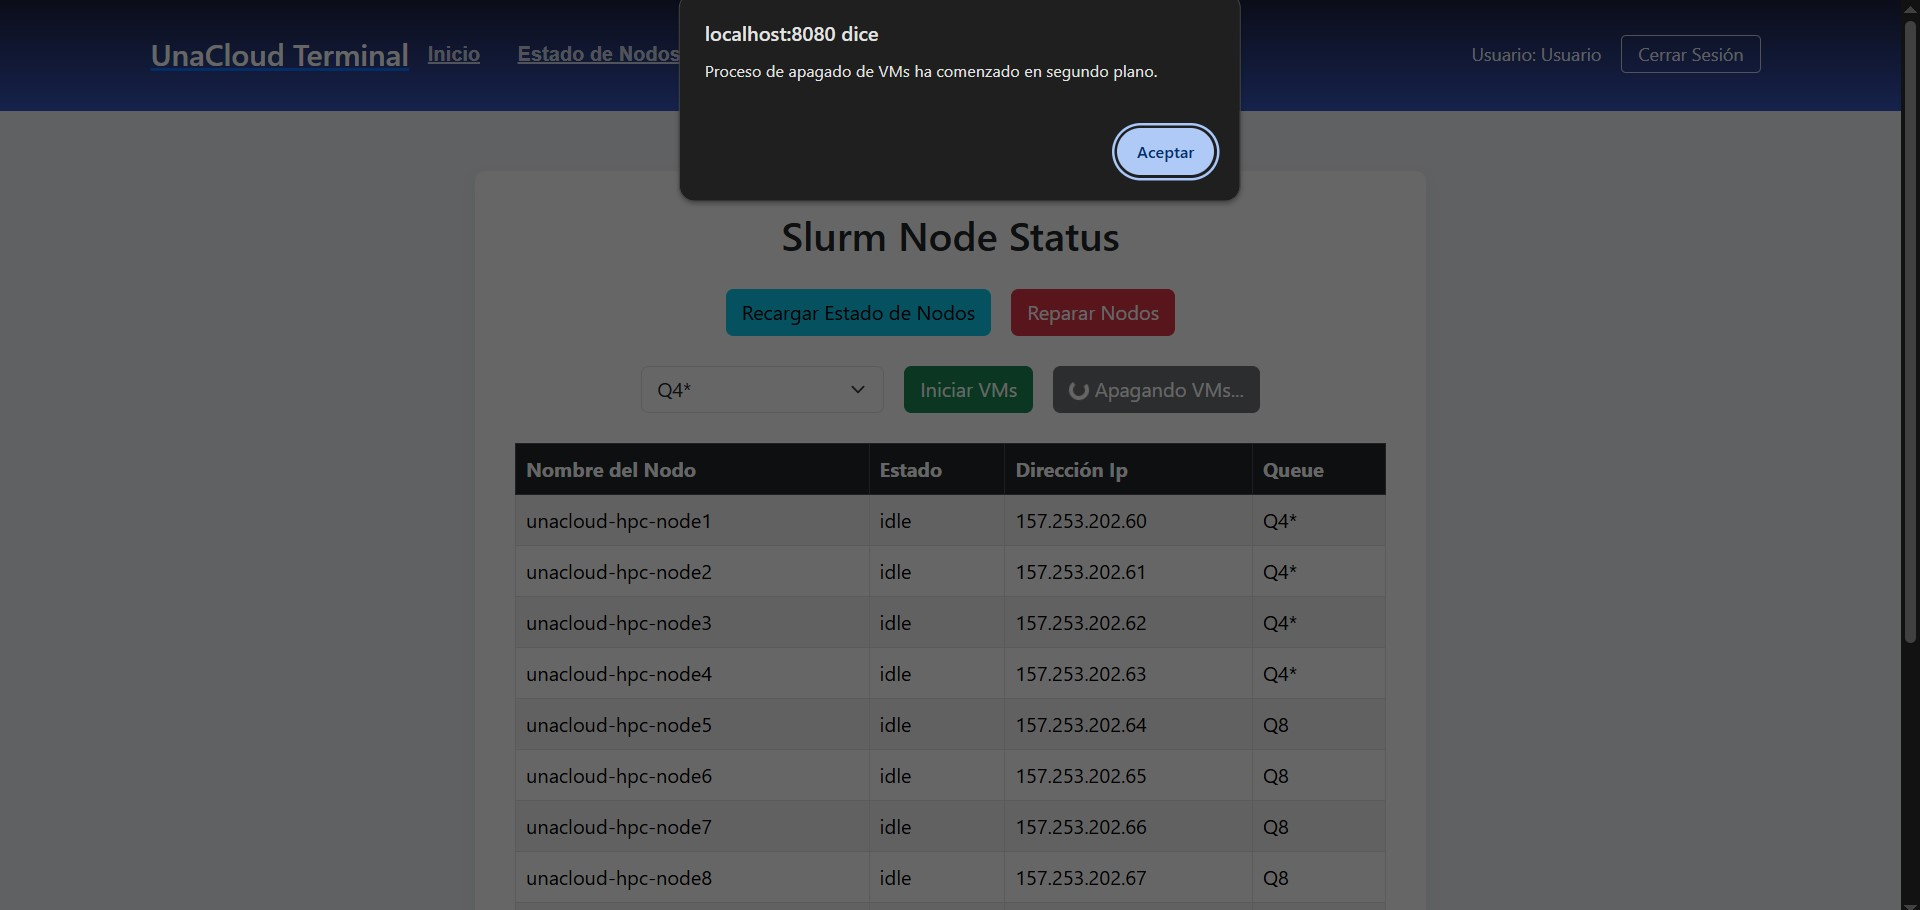
\includegraphics[width=0.75\linewidth]{Documento Final/Imagenes/ApagarNodosQ4.jpg}
    \caption{Proceso de apagado de las máquinas virtuales de la partición "Q4*". La interfaz notifica al usuario que el proceso de apagado ha comenzado en segundo plano.}
    \label{fig:NodeAdmin}
\end{figure}

\begin{figure}[H]
    \centering
    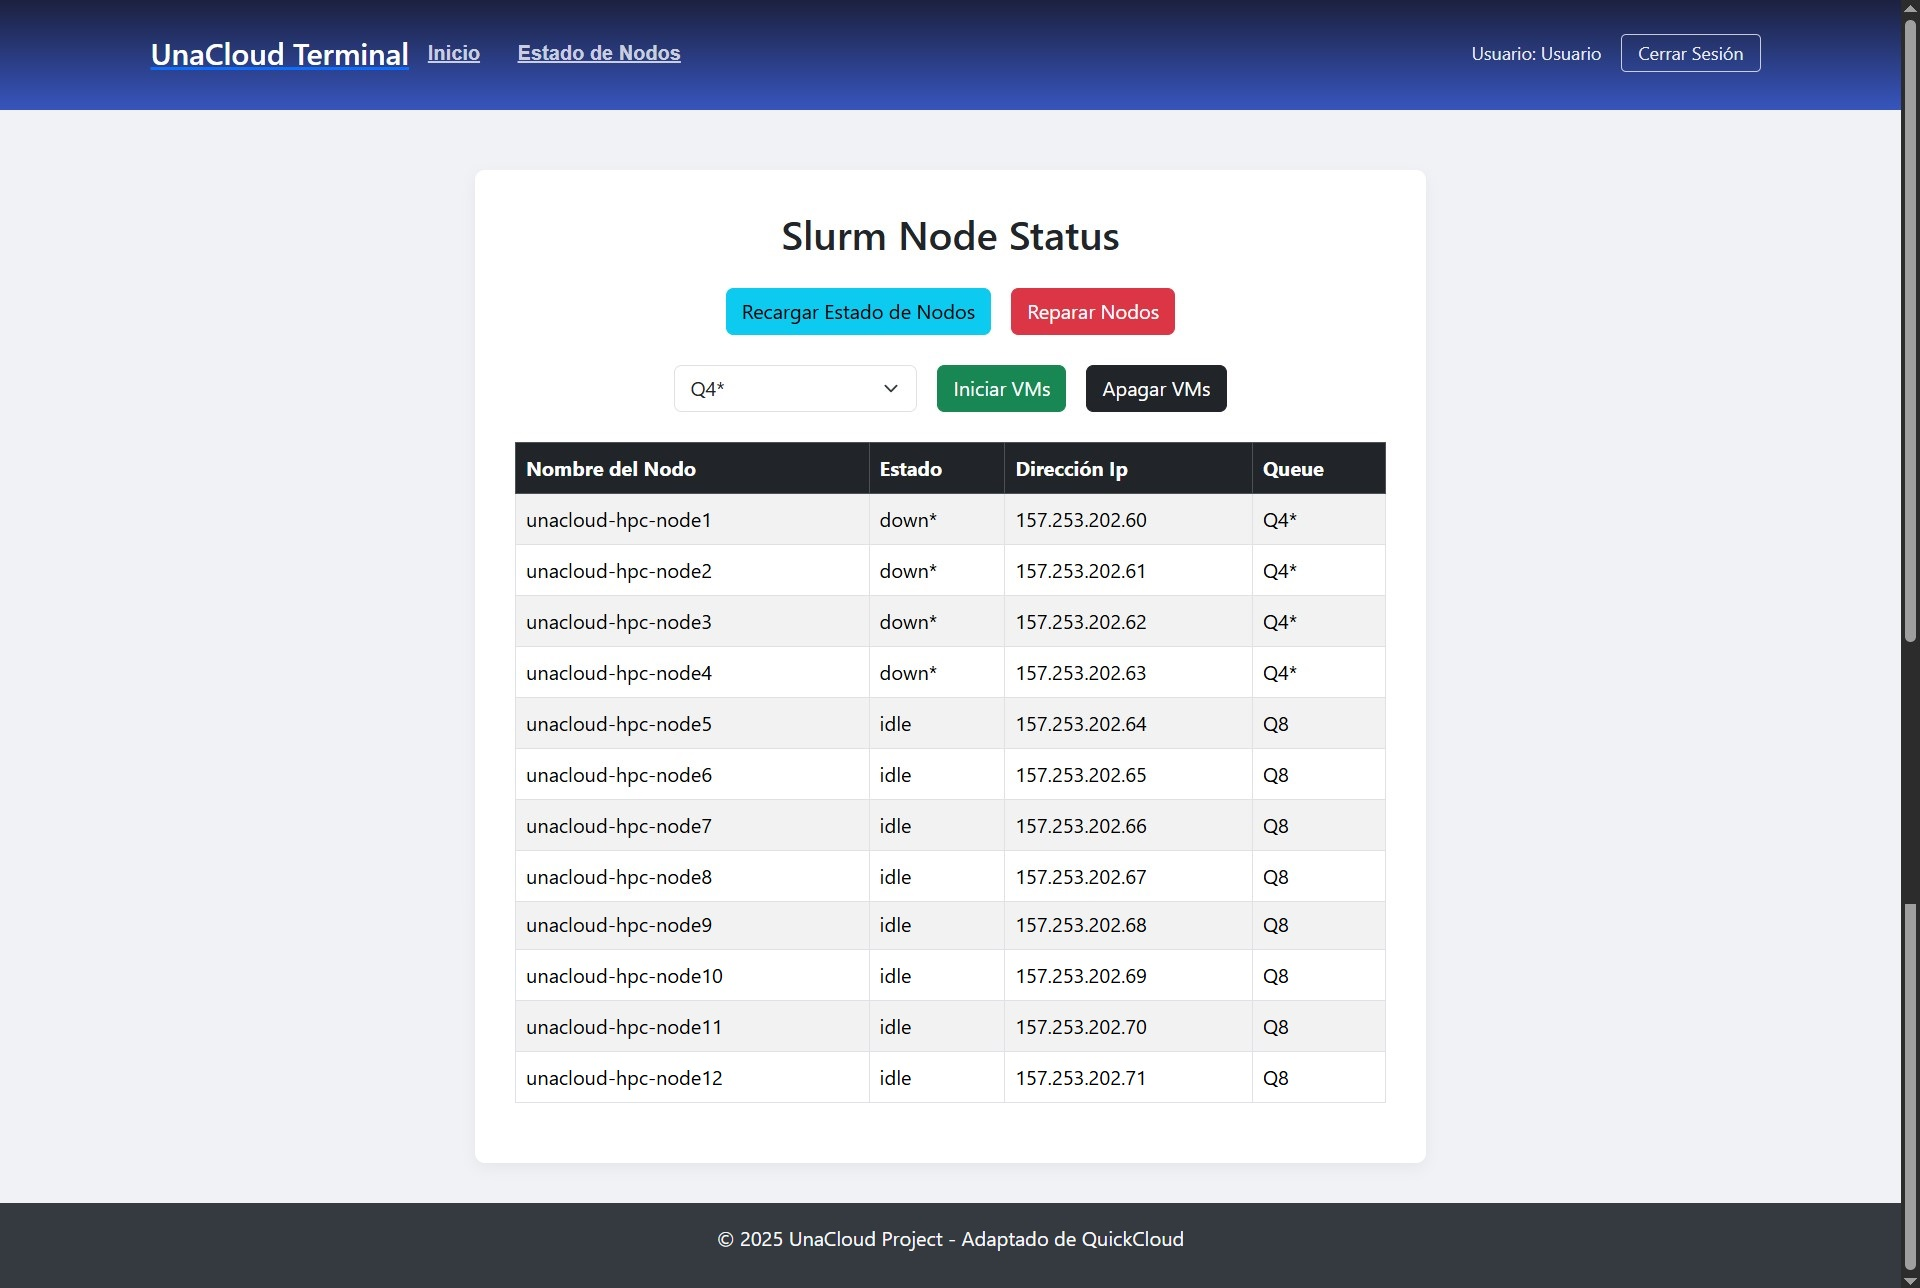
\includegraphics[width=0.75\linewidth]{Documento Final/Imagenes/NodosApagados.jpg}
    \caption{Vista del panel "Estado de Nodos" que muestra el resultado después de una operación de apagado sobre la partición "Q4*". El estado de los nodos unacloud-hpc-node1 a unacloud-hpc-node4 ha cambiado a down*, confirmando que sus máquinas virtuales han sido detenidas, mientras que los nodos de la partición Q8 permanecen activos (idle).}
    \label{fig:NodeState2}
\end{figure}


